\chapter{Numerical study of impact of vegetation on urban microclimate}
\label{ch:impactofvegetation}
\def\figdir{chapters/ch08_numericalstudy/figures}	
%\begin{quote} 
%	\begin{flushright}
%		\textit{The true logic of this world is in the\\ 
%			calculus of probabilities.}
%		
%		--- ~ James C. Maxwell
%	\end{flushright}
%\end{quote}

\section{Introduction}

In this chapter, the fully coupled (integrated) numerical model, described in \cref{ch:numericalmethod}, is used to assess the impact of vegetation on urban microclimate. To accurately assess the impact of vegetation on urban microclimate, we must determine: i) the influence of vegetation on the turbulent air flow, ii) the influence of plant transpiration on hygrothermal conditions, iii) the influence of plant shading on the urban environment, and iv), the net influence of all the parameters on the pedestrian thermal comfort. In this chapter, the influence of vegetation is assess using two different experimental setups: a) the study on the influence of vegetation on microclimate of a urban street canyon, and b) a case study on the influence of vegetation is a realistic city topology in Z\"urich, Switzerland at a location known as Muensterhof (in german: M\"unsterhof). The Muensterhof is a town square within the city of Zurich with that currently lacks vegetation. The objective of the study in the urban street canyon is to perform a parameteric study and determine the parameters that play a key role in improving the thermal comfort.  Furthermore, the influence of soil moisture change on the plant transpiration and the leaf energy balance is investigated. The objective of the case study in Muensterhof is determine the microclimate modification of vegetation in a realistic setting.

\section{Urban street canyon}

A numerical assessment of the impact of vegetation is first performed in urban street-canyon. The study investigates the influence of transpirative and shaded cooling due to vegetation on the pedestrian comfort inside a street canyon. In this study, we investigate the cooling potential of vegetation, such as a row of trees, on the microclimate of a street canyon using a CFD model in OpenFOAM. Prior to this study, the cooling effect of an isolated vegetation was studied in chapter in \cref{ch:parametricstudy}. In this study, we investigate the influence of vegetation in the setup described in \cite{Kubilay2018}, which investigated the influence of only the building on the microclimate. In this study,  we investigate how the microclimate is modified by the vegetation. The vegetation integrated numerical model is developed as as described in \cref{ch:numericalmethod} where the plant transpiration is dependent on the available soil moisture. Furthermore, vegetation modifies the street-canyon radiation balance as described in \cref{sec:radiationmodel}, where the vegetation intercepts the direct solar radiation and provides shading to the urban surfaces. The reflected (assumed to be diffused) short-wave radiation and long-wave radiation is modeled using surface-to-surface radiation model (i.e.,  \textit{radiosity} approach or also known as ``view factor'' model) as also described in  \cref{sec:radiationmodel}. The goal of a more advanced radiation treatment, in contrast to approach described in \cref{ch:parametricstudy}, is to provide a more accurate estimation of the mean radiant temperature $T_{\textit{mrt}}$, a key variable for an accurate prediction of thermal comfort index. In this study, the thermal comfort for pedestrians is evaluated using Universal Thermal Climate Index (UTCI). The aim of the study is to better understand the governing phenomena related to vegetation that plays a key role in improving the pedestrian thermal comfort. Therefore, the study simulates multiple cases to isolate the influence transpirative cooling and cooling due to shading by trees. Thus, we aim to understand the main contribution of natural cooling of vegetation on urban microclimate.  

\subsection{Simulation setup}

The simulations are performed for a street canyon with a vegetation zone of $2 \times 10 \times 4$ m$^3$, representing a row of trees which are surrounded by two buildings of $10 \times 50 \times 10$ m$^3$ ($x\times y \times z$), as shown in \cref{fig:domain_new5}. The numerical domain size is $230\times 250 \times 60$ m$^3$  ($x\times y \times z$), where the inlet, outlet, top, and side walls are positioned $5 H$, $5 H$, $15 H$, and $10 H$, respectively, based on CFD best practices \citep{Blocken2015, Franke2007, Tominaga2008}. The numerical domain is discretized into $\num{1178080}$ hexahedral cells with minimum cell size of $\num{1e-3}$ m$^{3}$ near the building walls (see \cref{fig:mesh_resolution}) and are determined following a grid-refinement study. The vegetation zone has a foliage height of $4$ m (with $z_{\textit{min}}= 4$ m), leaf area density $a= 1$ m$^2$\,m$^{-3}$, leaf drag coefficient $c_d=0.2$ and leaf size $l=0.1$ m. The building are oriented perpendicular to the wind direction. The meteorological data are based on a typical meteorological year and the total solar radiation intensity is for a clear sky on the 21$^{\mathrm{st}}$ of June in the city of Zurich, Switzerland used in the study of \cite{Kubilay2018}. The wind speed at the building height is $U_{\textit{ref}}=5$ m\,s$^{-1}$ where turbulence kinetic energy $k$ and turbulence dissipation rate $\varepsilon$ are determined using \cref{eq:ableq} \citep{Richards1993} with $u_*/U = 0.072$ and $z_0 = 0.03$ m. Standard wall functions are employed for the wall boundary and a constant static pressure of $p=0$ Pa at the outlet boundary. The inlet, top and side wall are prescribed with the ambient temperature varies between 11$^{\circ}C$ and 19 $^{\circ}C$ with solar noon at $13:28$ and the relative humidity varies between 62\% and 86\% $RH$ as shown in \cref{fig:meteobc}. The ambient CO$_2$ concentration is taken to be $c=380$ $\mu$mol\,mol$^{-1}$. 

	\begin{figure}[t]
	\centering
	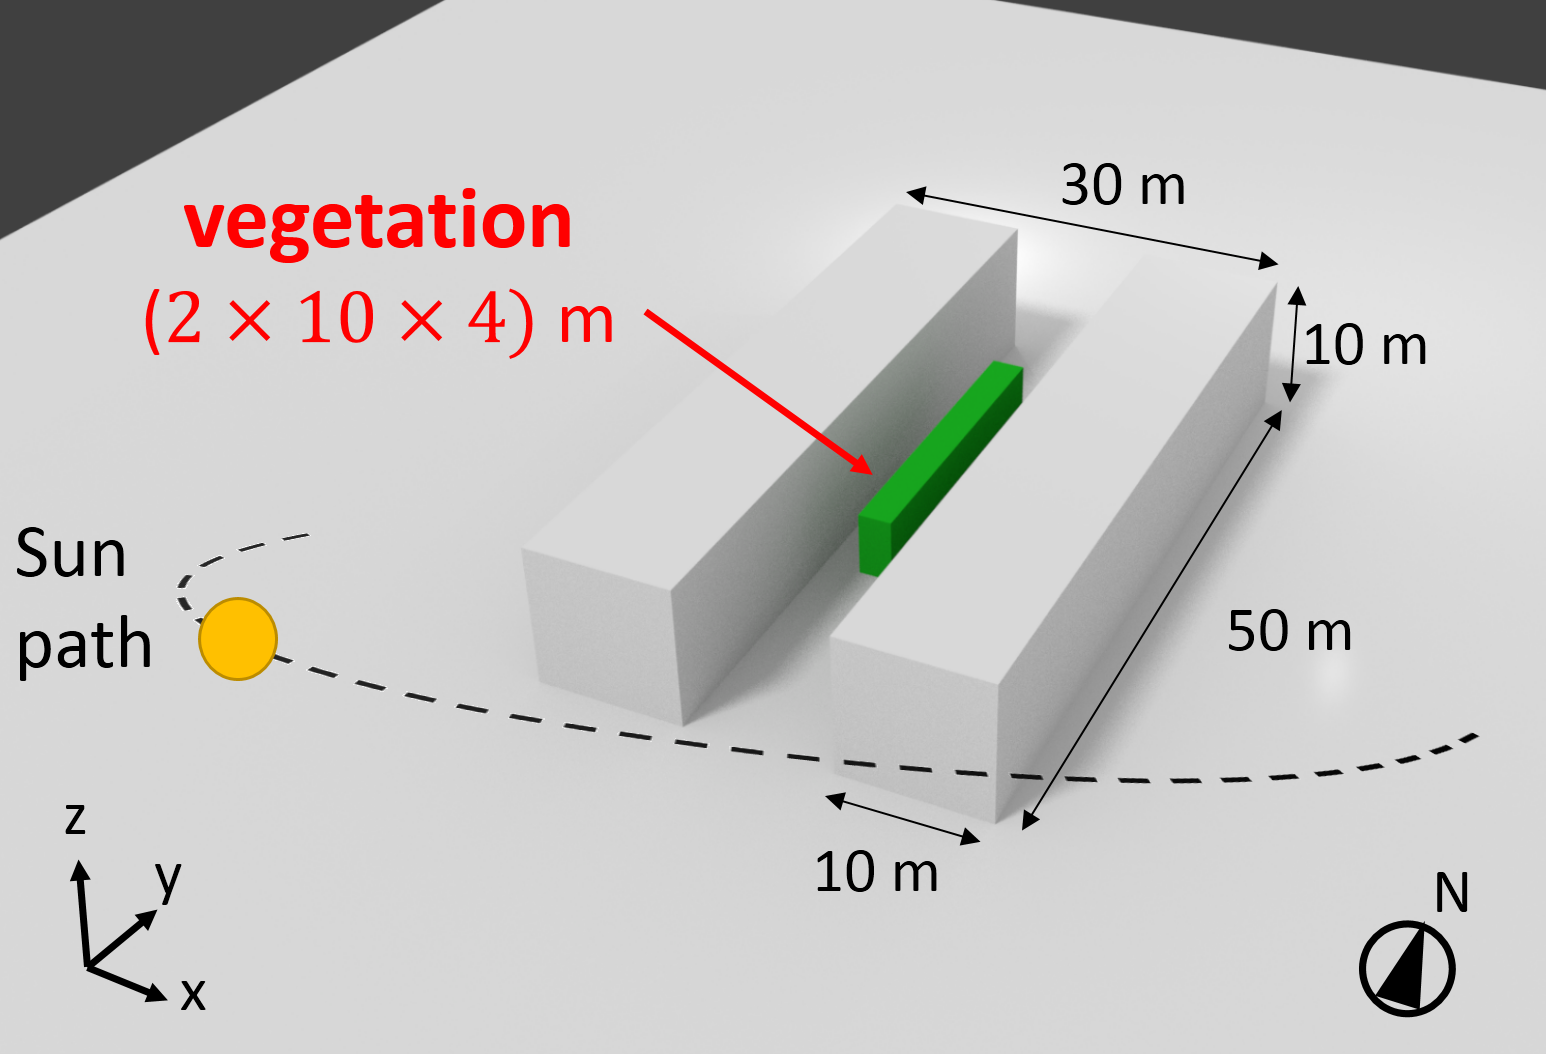
\includegraphics[width=0.8\textwidth]{\figdir/domain_new5.png}
	%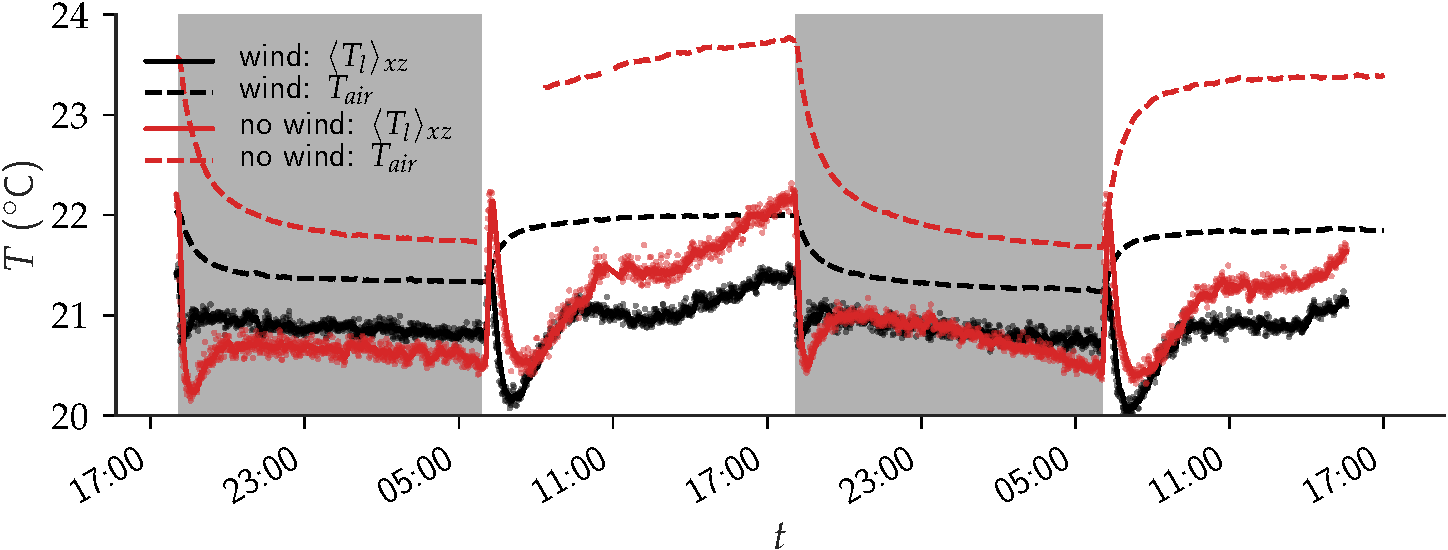
\includegraphics[width=\textwidth]{\figdir/Tinfrared_vs_air_updated-crop.pdf}
	\caption{The simulation setup of a street canyon composed of two buildings measuring $10 \times 50 \times 10$ m$^3$ ($x\times y \times z$) with vegetation band of size $2 \times 10 \times 4$ m$^3$ in the center. The setup is based on the study of Kubilay et al. (2017) with wind.}
	\label{fig:domain_new5}
	\end{figure}


\begin{figure}[p]
	\centering
	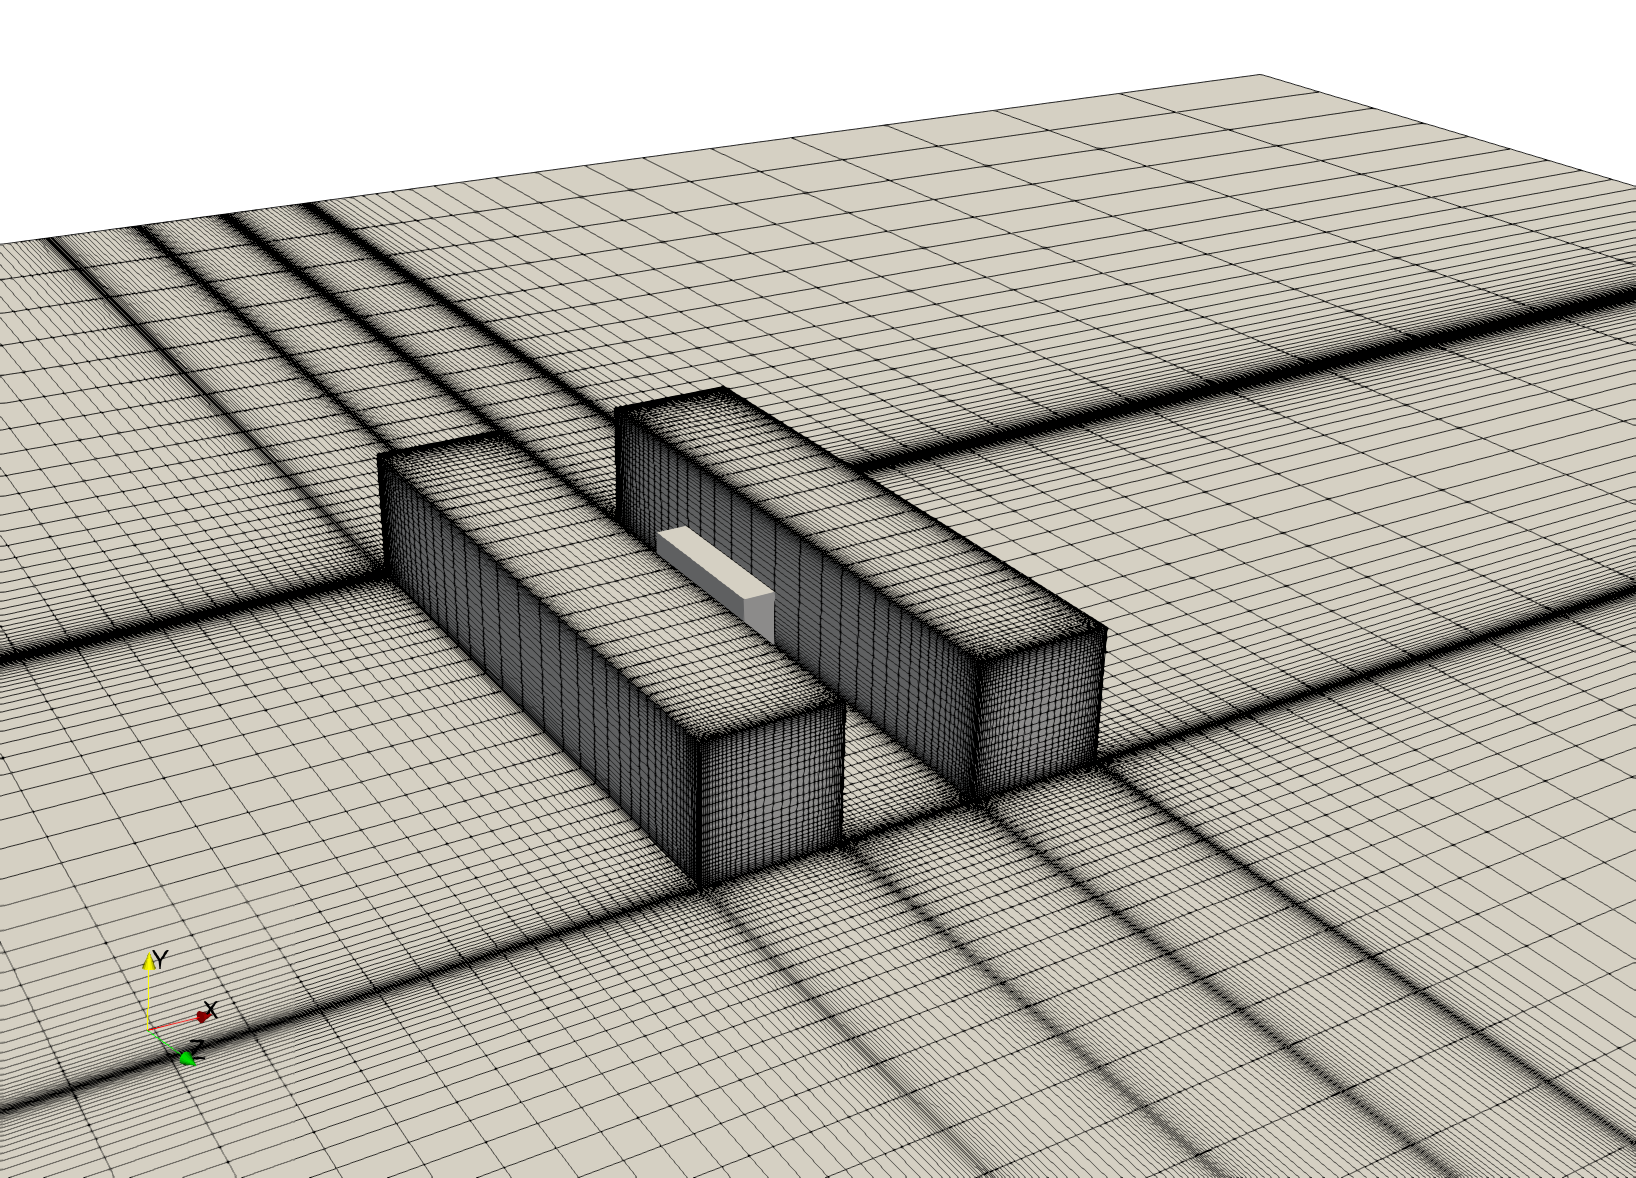
\includegraphics[width=0.6\textwidth]{\figdir/mesh_resolution.png}
	%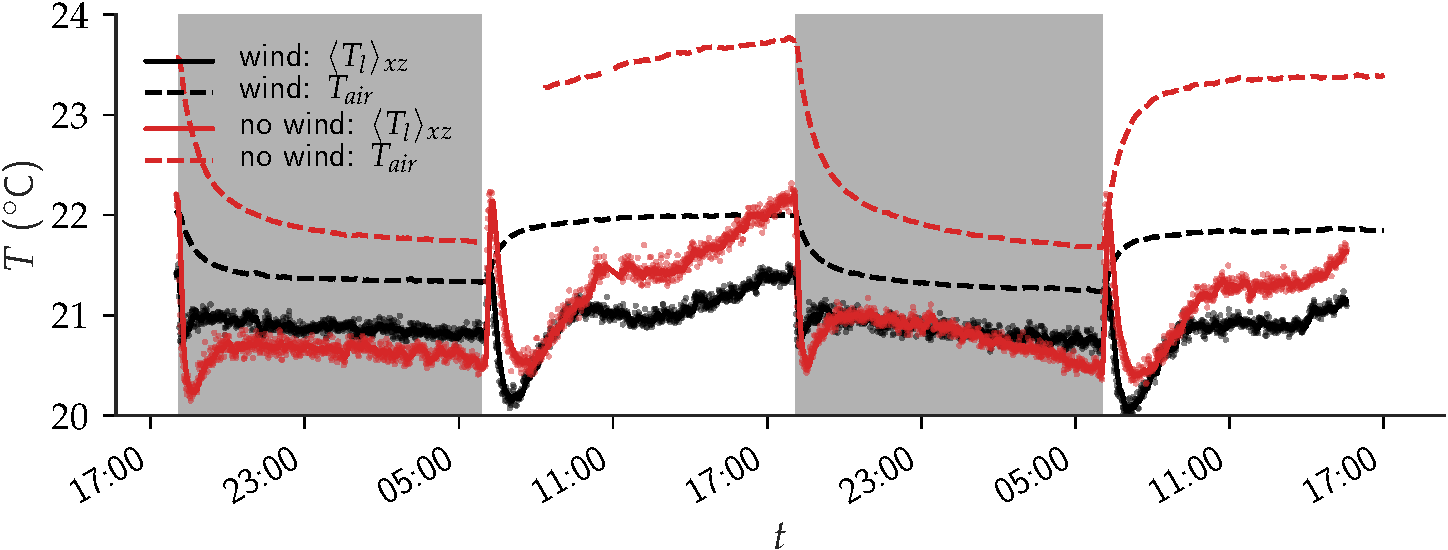
\includegraphics[width=\textwidth]{\figdir/Tinfrared_vs_air_updated-crop.pdf}
	\caption{Simulation domain showing the surface layer mesh refined closed to the building walls. The numerical domain is discretized into $\num{1178080}$ hexahedral cells with minimum cell size of $\num{1e-3}$ m$^{3}$ at the building corner. The mesh is based on the grid refinement study of \cite{Kubilay2018}.}
	\label{fig:mesh_resolution}
\end{figure}

\begin{figure}[p]
	\centering
	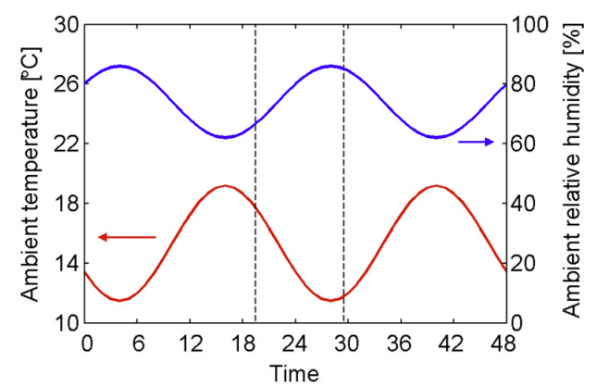
\includegraphics[width=0.8\textwidth]{\figdir/meteobc.png}
	%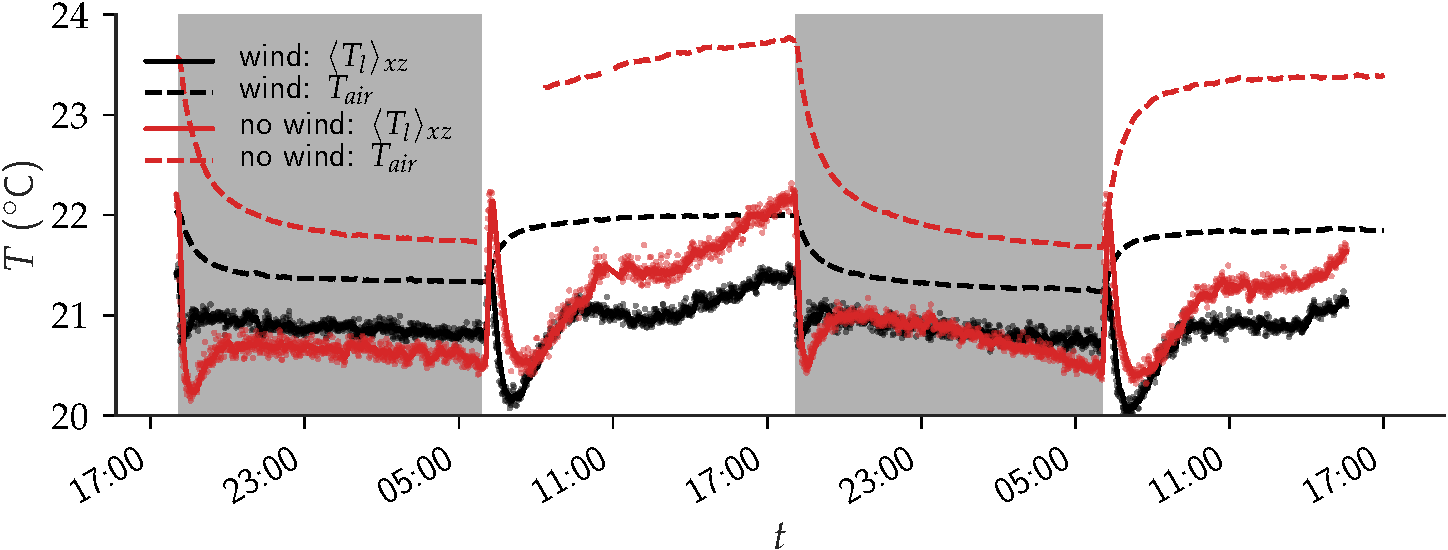
\includegraphics[width=\textwidth]{\figdir/Tinfrared_vs_air_updated-crop.pdf}
	\caption{Diurnal ambient temperature $T$ ($^{\circ}C$) and relative humidity $RH$ (\%) profile obtained from \cite{Kubilay2018}. The meteorological data are based on a typical meteorological year and the total solar radiation intensity is for a clear sky on the 21$^{\mathrm{st}}$ of June in the city of Z\"urich, Switzerland. }
	\label{fig:meteobc}
\end{figure}

\begin{figure}[p]
	\centering
	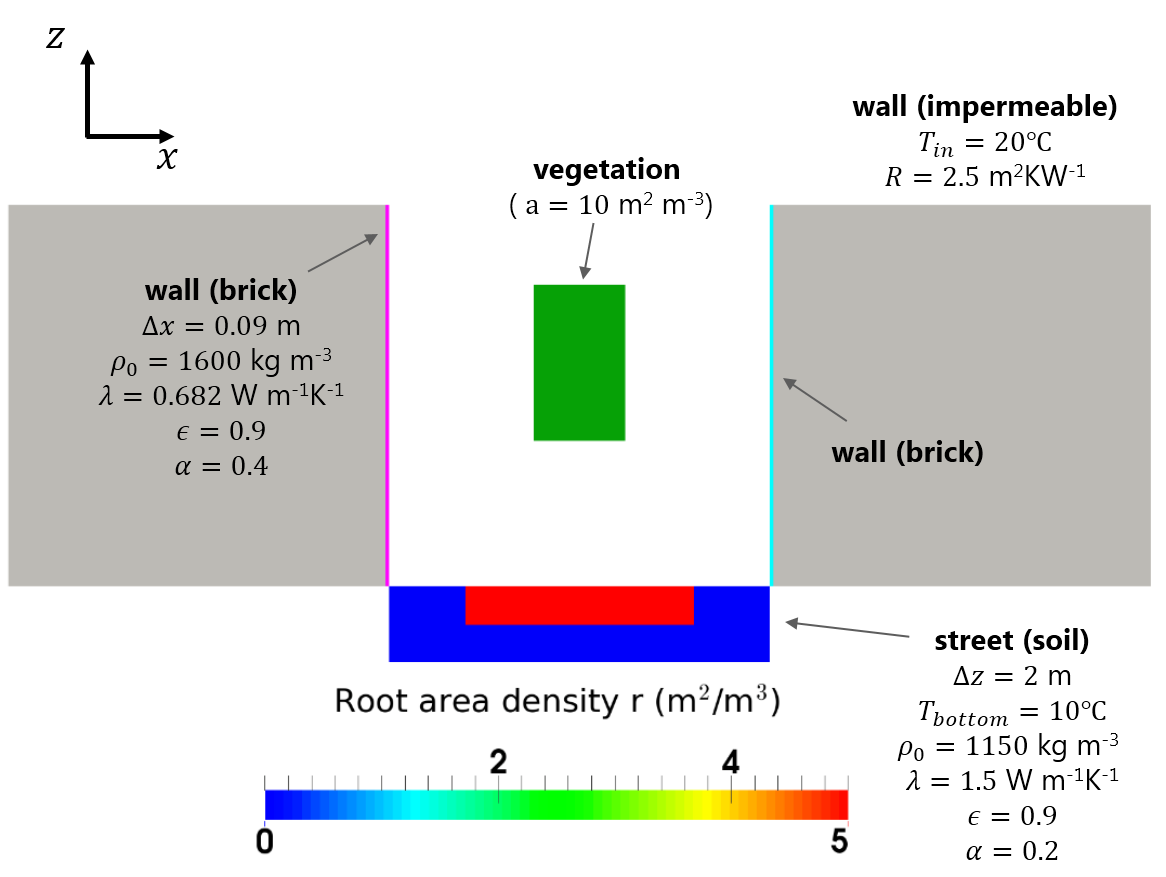
\includegraphics[width=\textwidth]{\figdir/soliddomain_v2.png}
	%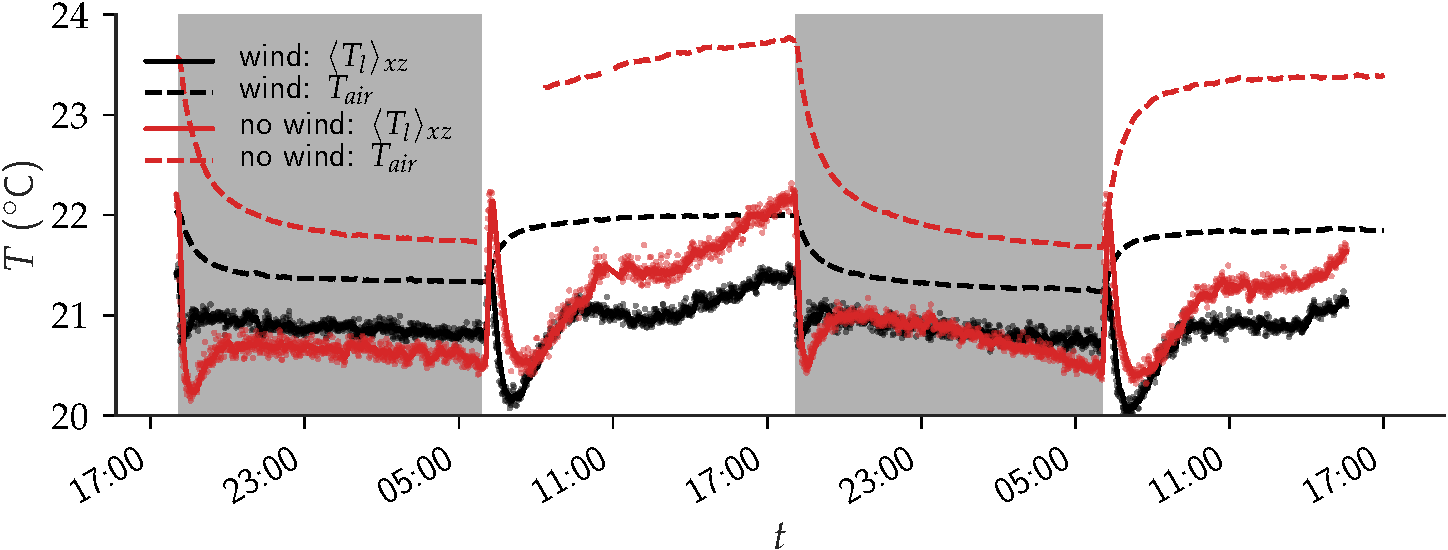
\includegraphics[width=\textwidth]{\figdir/Tinfrared_vs_air_updated-crop.pdf}
	\caption{Description of the solid domain consisting of two impervious buildings of size $10 \times 50 \times 10$ m$^3$ ($x\times y \times z$) each with a brick layer of $0.09$ m inside the street-canyon and a soil region at the street with vegetation roots. The temperature $T_{\textit{in}}$, thermal resistance $R$, the density $\rho_0$, thermal conductivity $\lambda$, emissivity $\epsilon$, albedo $\alpha$, leaf area density $a$ and root area density $r$ and also provided. }
	\label{fig:soliddomain}
\end{figure}


\ctable[
caption = {Soil-plant-atmosphere continuum (SPAC) vegetation parameters of Loblolly pine (\textit{Pinus taeda}) are used in the study obtained from \citep{Manoli2014,Volpe2013,Launiainen2015,Manzoni2011,Vogel2016}},
label   = {tab:spacconditions},
pos = p,
mincapwidth = \textwidth,
]{llrl}{}{
	\FL
	Parameter					& Description 				& Value  & Unit
	\ML
	$c$						 	& Ambient CO$_2$ concentration & $380$ & $\mu$mol\,mol$^{-1}$		\\
	$c_*$						 	&  CO$_2$ concentration at max. WUE & $400$ & $\mu$mol\,mol$^{-1}$		\\
	$c_o$						& Ambient O$_2$ concentration & $210$ & mmol\,mol$^{-1}$		\\
	$a$  							& leaf area density		& $1$ &m$^{2}$\,m$^{-3}$\\
	$l$								 & leaf size				 & $0.1$ &m \\	
	
	$\lambda_{\textit{max}}$ & Maximum WUE 	 & $2912$ &$\mu$mol\,mol$^{-1}$	\\
	$\beta_{L}$ &  WUE coefficient & $\num{0.78e-12}$ & \\	
	$\psi_{L}^{\textit{max}}$ &  leaf water potential at max. WUE & $\num{-1.85e-6}$ &Pa\\	
	$k_x$ &  xylem conductance & $\num{5e-6}$ &s$^{-1}$\\	
	$A_x$ &  xylem cross-section area & $0.06$ &m$^{2}$\\
	$k_{\textit{st,n}}$			& nocturnal stomatal conductance & $0.018$ &mol\,m$^{-2}$\,s$^{-1}$ \\	
	$r$ 							 & root area density 	& $5$ &m$^{2}$\,m$^{-3}$	 \\
	$r_{\textit{radius}}$		& root radius 			  & $0.02$ &m \\
	$\beta$						 & soil conductance coefficient & $\num{3e8}$ &\\
	$k_r$							& root conductance 	& $\num{3e-11}$ &s$^{-1}$ \\
	
	\LL}

The coupling of air domain, the solid domains (including soil region), with the vegetation is discussed in \cref{sec:couplingalgorithm}. \cref{fig:soliddomain} shows the setup of the solid domain used in the study. The figure depicts configuration of two buildings forming a street-canyon with a vegetation zone in the middle. The cross-section is a $x-z$ plane at $y=125$ m  (i.e., $y$-center of the street-canyon). The two impervious buildings has a size $10 \times 50 \times 10$ m$^3$ ($x\times y \times z$) each with a brick layer of $0.09$ m inside the street-canyon and a soil region at the street where the vegetation roots is present. The soil is composed of equal composition of sand, silt, and clay with a uniform root area density $r = 5$ m$^{2}$\,m$^{-3}$ of the size of $4 \times 14 \times 1$ m$^{3}$ directly below the foliage region, spanning $\mvec{x}_{\textit{min}} = (62, -1, 118)$ and $\mvec{x}_{\textit{max}} = (68, 0, 132)$. The temperature $T_{\textit{in}}$, thermal resistance $R$, the density $\rho_0$, thermal conductivity $\lambda$, emissivity $\epsilon$ and albedo $\alpha$ of the various solid regions are also indicated in \cref{fig:soliddomain}. The vegetation parameters used in the soil-plant-atmosphere continuum (SPAC) vegetation model is given in \cref{tab:spacconditions}. The vegetation properties are based of Loblolly pine (\textit{Pinus taeda}) \citep{Manoli2014,Volpe2013,Launiainen2015,Manzoni2011,Vogel2016}. In future, this numerical modeling approach should enables to study various other species that are more common in cities.

\subsection{Results and Discussion}

%The influence of vegetation on the microclimate of the street canyon (depicted in Fig.1) is studied using the developed numerical model. The natural cooling provided by the row of trees is determined by comparing the setup with and without vegetation, “V” and “NV”, respectively. Fig. 2 shows the change in air temperature, $T_v-T_nv$ at noon (12 pm), when the sun is directly above the street canyon. The vegetated region is indicated by the dashed outline. From the figure, two distinct regions of cool zones can be identified. The first region is at the vicinity of the vegetation with a temperature change of around -2 . This cool zone results from the transpirative cooling effect of vegetation. 

%The second zone is the region close to the building wall, where the shadow of the tree was present earlier during the day. This cooling region, resulting from tree shading, is seen to be more effective than the transpirative cooling region, showing a temperature drop of more than -3. Furthermore, at the current location of the shadow, the cooling air is seen to be convected away from the wall, and interacts with the cool zone. This indicates that, in addition to transpirative cooling, the tree-shade cooling plays a vital role in improving the microclimate. It is also evident that, as a result of the combined influence of transpirative and tree-shade cooling, the overall surface temperature of the street canyon is lower.


The influence of vegetation in an urban street canyon is determined by separately studying the influence of shading and the plant transpiration. The influence of these two parameters on the microclimate inside the street-canyon is studied by determined the influence on air temperature, mean radiation temperature, short-wave radiation intensity, and finally UTCI distribution. 

\subsubsection*{Influence of plant transpiration and shading}

\cref{fig:USC_T} shows the direct short-wave radiation intensity $|q_{\textit{s,dir}}|$ (W\,m$^{-2}$) inside the street-canyon (i.e., $x-z$ plane at $y=125$ m) where the vegetation zone is indicated by a green box. Nine subplot at shown of different times of the days from $03$:$00$ (HH:MM) to $23$:$00$ (HH:MM) with $150$ minutes interval. The figure shows the contribution of the vegetation to the solar radiation intensity inside the street-canyon. We see that vegetation intercepts the solar radiation during the day providing shading to the nearby urban surfaces. The vegetation acts as a radiation sink especially when the solar radiation is high during noon. This is important as the urban materials with high thermal capacity, contributes to the urban heat island by absorbing the solar radiation. By providing shading to the urban environment, vegetation can therefore mitigate the urban heat island effect.  

\begin{sidewaysfigure}[p]
	\centering
	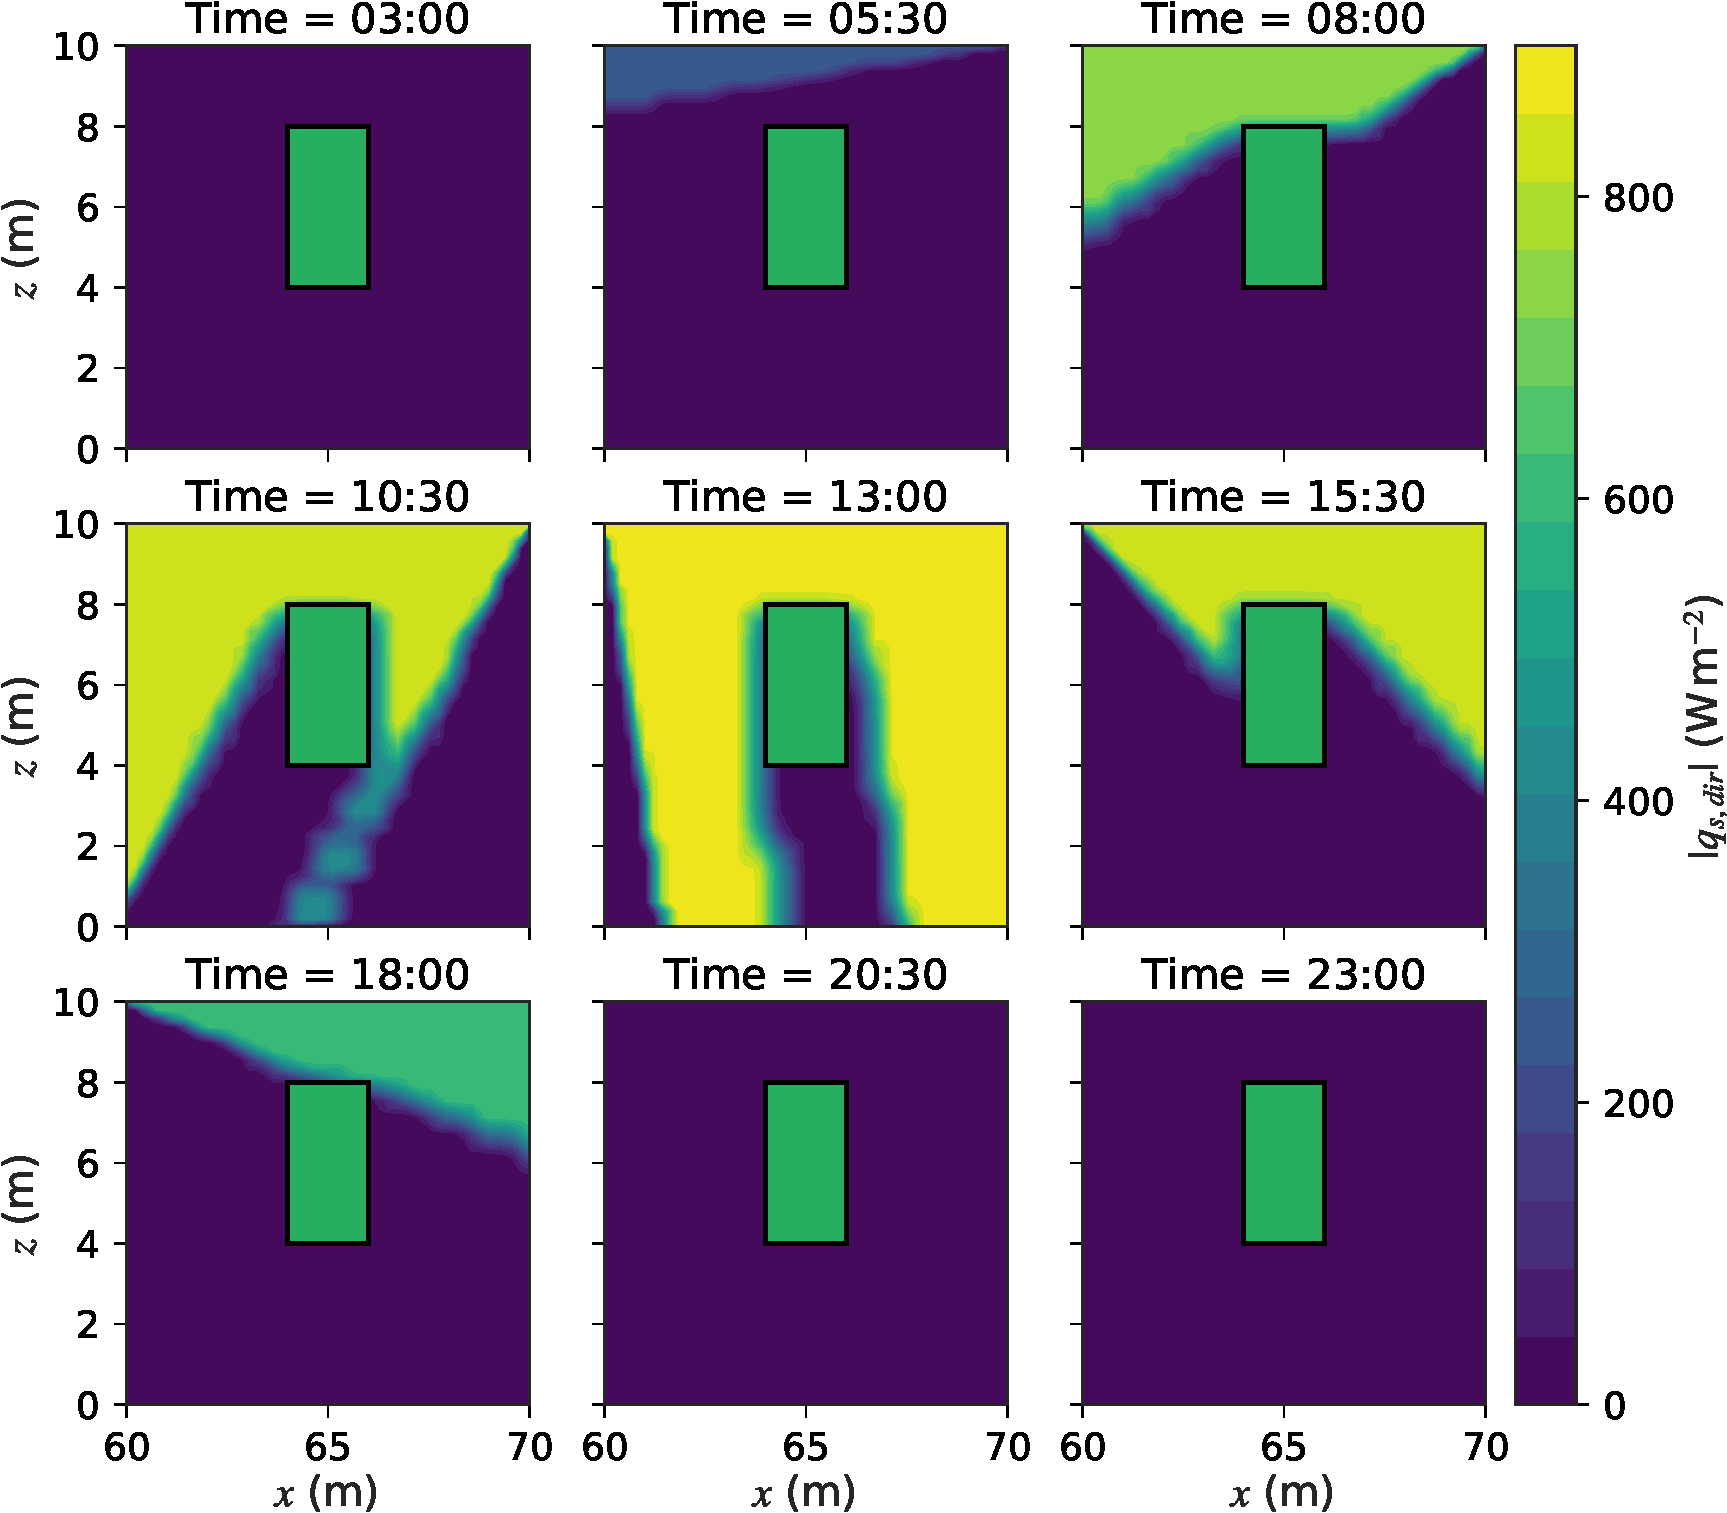
\includegraphics[width=0.8\textwidth]{\figdir/USC_qsdir-crop.pdf}
	\caption{Direct short-wave radiation intensity $|q_{\textit{s,dir}}|$ (W\,m$^{-2}$) inside the street-canyon where the vegetation zone is indicated by a green box. The plot shows the fields with a $150$ minutes interval from $03$:$00$ (HH:MM) to $23$:$00$ (HH:MM).}
	\label{fig:USC_qrdir}
\end{sidewaysfigure}

\begin{sidewaysfigure}[p]
	\centering
	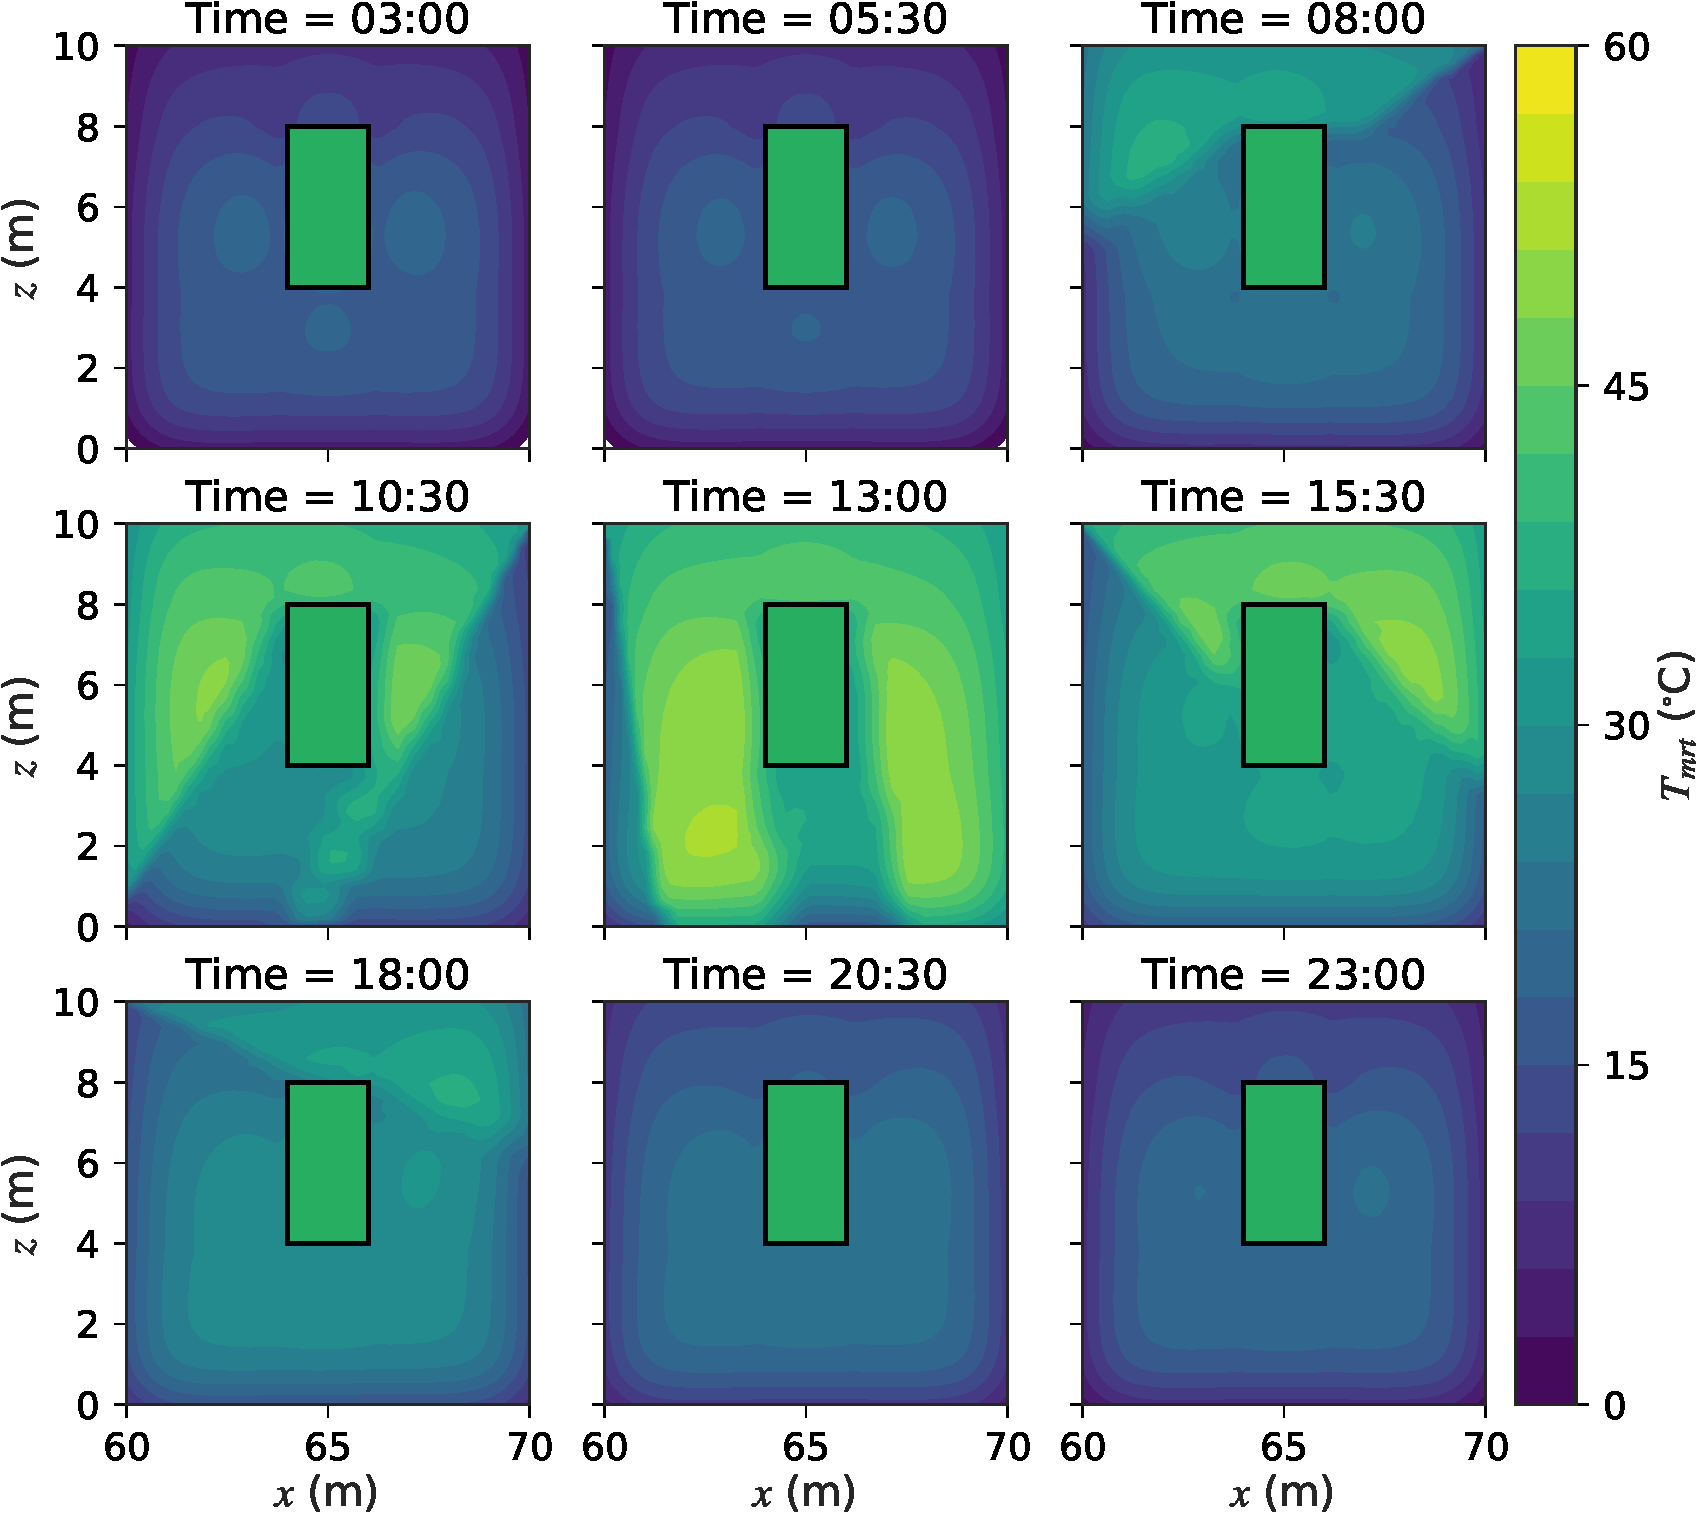
\includegraphics[width=0.8\textwidth]{\figdir/USC_Tmrt-crop.pdf}
	\caption{Mean radiant temperature $T_{\textit{mrt}}$  ($^{\circ}$C) inside the street-canyon where the vegetation zone is indicated by a green box. The plot shows the fields with a $150$ minutes interval from $03$:$00$ (HH:MM) to $23$:$00$ (HH:MM).}
	\label{fig:USC_Tmrt}
\end{sidewaysfigure}


\cref{fig:USC_Tmrt} shows the mean radiant temperature $T_{\textit{mrt}}$  ($^{\circ}$C) inside the street-canyon throughout the day. The mean radiant temperature is determined as follows: 
\begin{equation}
T_{\textit{mrt}} = \left( T_{\textit{umrt}}^4  + \frac{f_p a_b}{\epsilon_p \sigma} q_{\textit{s,dir}} \right)^{\frac{1}{4}}
\label{eq:Tmrt2}
\end{equation}
where $T_{\textit{umrt}}$ is the mean radiant temperature component belonging to the diffused or reflected part (i.e., from terrestrial source), $f_p$ is projected surface area of the person exposed to the sun, $\alpha_p$ is the albedo, $\epsilon_p$ is the emission coefficient and $q_{\textit{s,dir}}$ (W\,m$^{-2}$) is the direct solar radiation. The diffused/reflected component of the MRT is defined as:
\begin{equation}
T_{\textit{umrt}} = \left[ \frac{1}{\sigma} \sum_{i}^N \left(q_{\textit{r,i}} + \frac{a_b}{\epsilon_p} q_{\textit{s,i}} \right)F_i\right]^{\frac{1}{4}}
\label{eq:Tumrt2}
\end{equation}
where $q_{\textit{r,i}}$ (W\,m$^{-2}$)  is the long-wave radiation emitted from surface $i$, $q_{\textit{s,i}}$ (W\,m$^{-2}$) is the reflected (assumed to be diffused) short-wave radiation from surface $i$, and $F_i$ is the view-factor between surface $i$ and the person. Thus, the mean radiant temperature $T_{\textit{mrt}}$ is directly dependent on the long-wave and the short-wave radiation fluxes in the street-canyon, including the contribution from the direct solar radiation $q_{\textit{r,dir}}$. \cref{fig:USC_Tmrt} is seen to be directly correlated with the short-wave radiation plots depicted in \cref{fig:USC_qrdir}. At regions of high direct solar radiation, the mean radiant temperature approach $T_{\textit{mrt}}\rightarrow50$ ($^{\circ}$C). In the shaded regions, there is a $18$  ($^{\circ}$C) difference in the mean radiant temperature. This indicates that solar radiation plays a crucial role in the mean radiant temperature and thereby the thermal comfort (investigated in detail in the next section). Furthermore, we see that pedestrian level (i.e., $z=2$ m) the mean radiant temperature is at highest. This is related to the emitted (or reflected) radiation from urban surfaces. At the height of $2$ m, the location is exposed to (or ``views'') more urban surfaces with emit the radiation. Therefore, the diffused radiation from the building surfaces also has a contributing effect on the mean radiant temperature. During night-time, we see that the mean radiant temperature gradually reduces. This is due to the nocturnal radiation cooling, where the long-wave radiation from the building surfaces is emitted to the atmosphere during night, thereby cooling the building surfaces. A trapping of this radiation such as due to cloud cover or even the presence of vegetation could negatively effect the noctural radiation cooling. 

\begin{figure}[t]
	\centering
	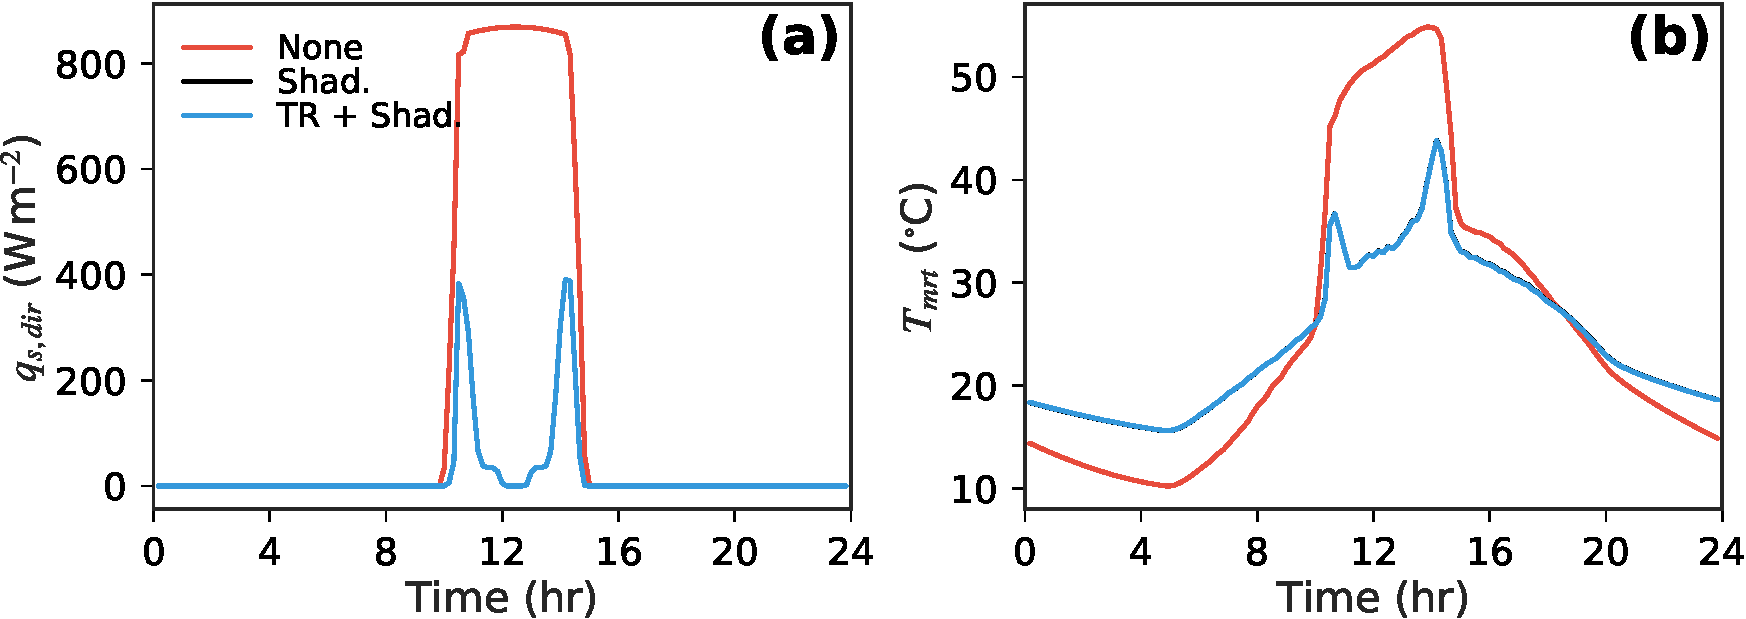
\includegraphics[width=\textwidth]{\figdir/profile_qsdir_Tmrt-crop.pdf}
	\caption{Diurnal profile below the tree at $(x,y,z) = (65, 125, 2)$ comparing three cases: no vegetation (\textit{None}), vegetation with only shading (\textit{Shad.}), and vegetation providing shading and transpirative cooling (\textit{TR + Shad.}): \subfig{a} direct short-wave radiation intensity $\left\|q_{\textit{s,dir}}\right\|T$ (W\,m$^{-2}$) and \subfig{b} mean radiant temperature $T_{\textit{mrt}}$  ($^{\circ}$C). }
	\label{fig:profile_qsdir_Tmrt}
\end{figure}

To better investigate the impact of plant shading and the changes in mean radiant temperature in the street-canyon due to vegetation, a single point below the tree at $(x,y,z) = (65, 125, 2)$ is investigated for three difference cases: the configuration without vegetation (\textit{None}), the configuration with vegetation but providing only shading (\textit{Shad.}), and the configuration with vegetation providing both and plant transpiration (\textit{TR + Shad.}), \cref{fig:profile_qsdir_Tmrt}. \cref{fig:profile_qsdir_Tmrt}a shows the diurnal variation of the direct short-wave radiation intensity $\left\|q_{\textit{s,dir}}\right\|T$ (W\,m$^{-2}$) below the tree. At the presence of vegetation, we see a strong drop in the solar radiation, especially during mid days from $q_{dir} \approx 800$ W\,m$^{-2}$ to zero at mid day and slightly above zero when the sun is off the solar noon. Therefore, all the solar radiation is intercepted by the foliage provide a strong shading below the tree. The dirunal profile of the mean radiant temperature $T_{\textit{mrt}}$  ($^{\circ}$C), \cref{fig:profile_qsdir_Tmrt}b, shows that shading provides up to $\approx 20$ drop when shaded. This is especially beneficial as the the largest temperature drop is prevalent the mean radiant temperature would have been highest during the day. Thus, shading provided could be vital component in improving the pedestrian thermal comfort. A detailed investigation on the impact of shading on UTCI is performed in th next section. At night we see that the vegetation instead increases the mean radiant temperature inside the street-canyon. This occurs because vegetation results in the radiation trapping it intercepts the long-wave radiation emitted from the urban surfaces to the sky. This phenomena could therefore have a negative effect on the thermal comfort during night time. 

\begin{sidewaysfigure}[p]
	\centering
	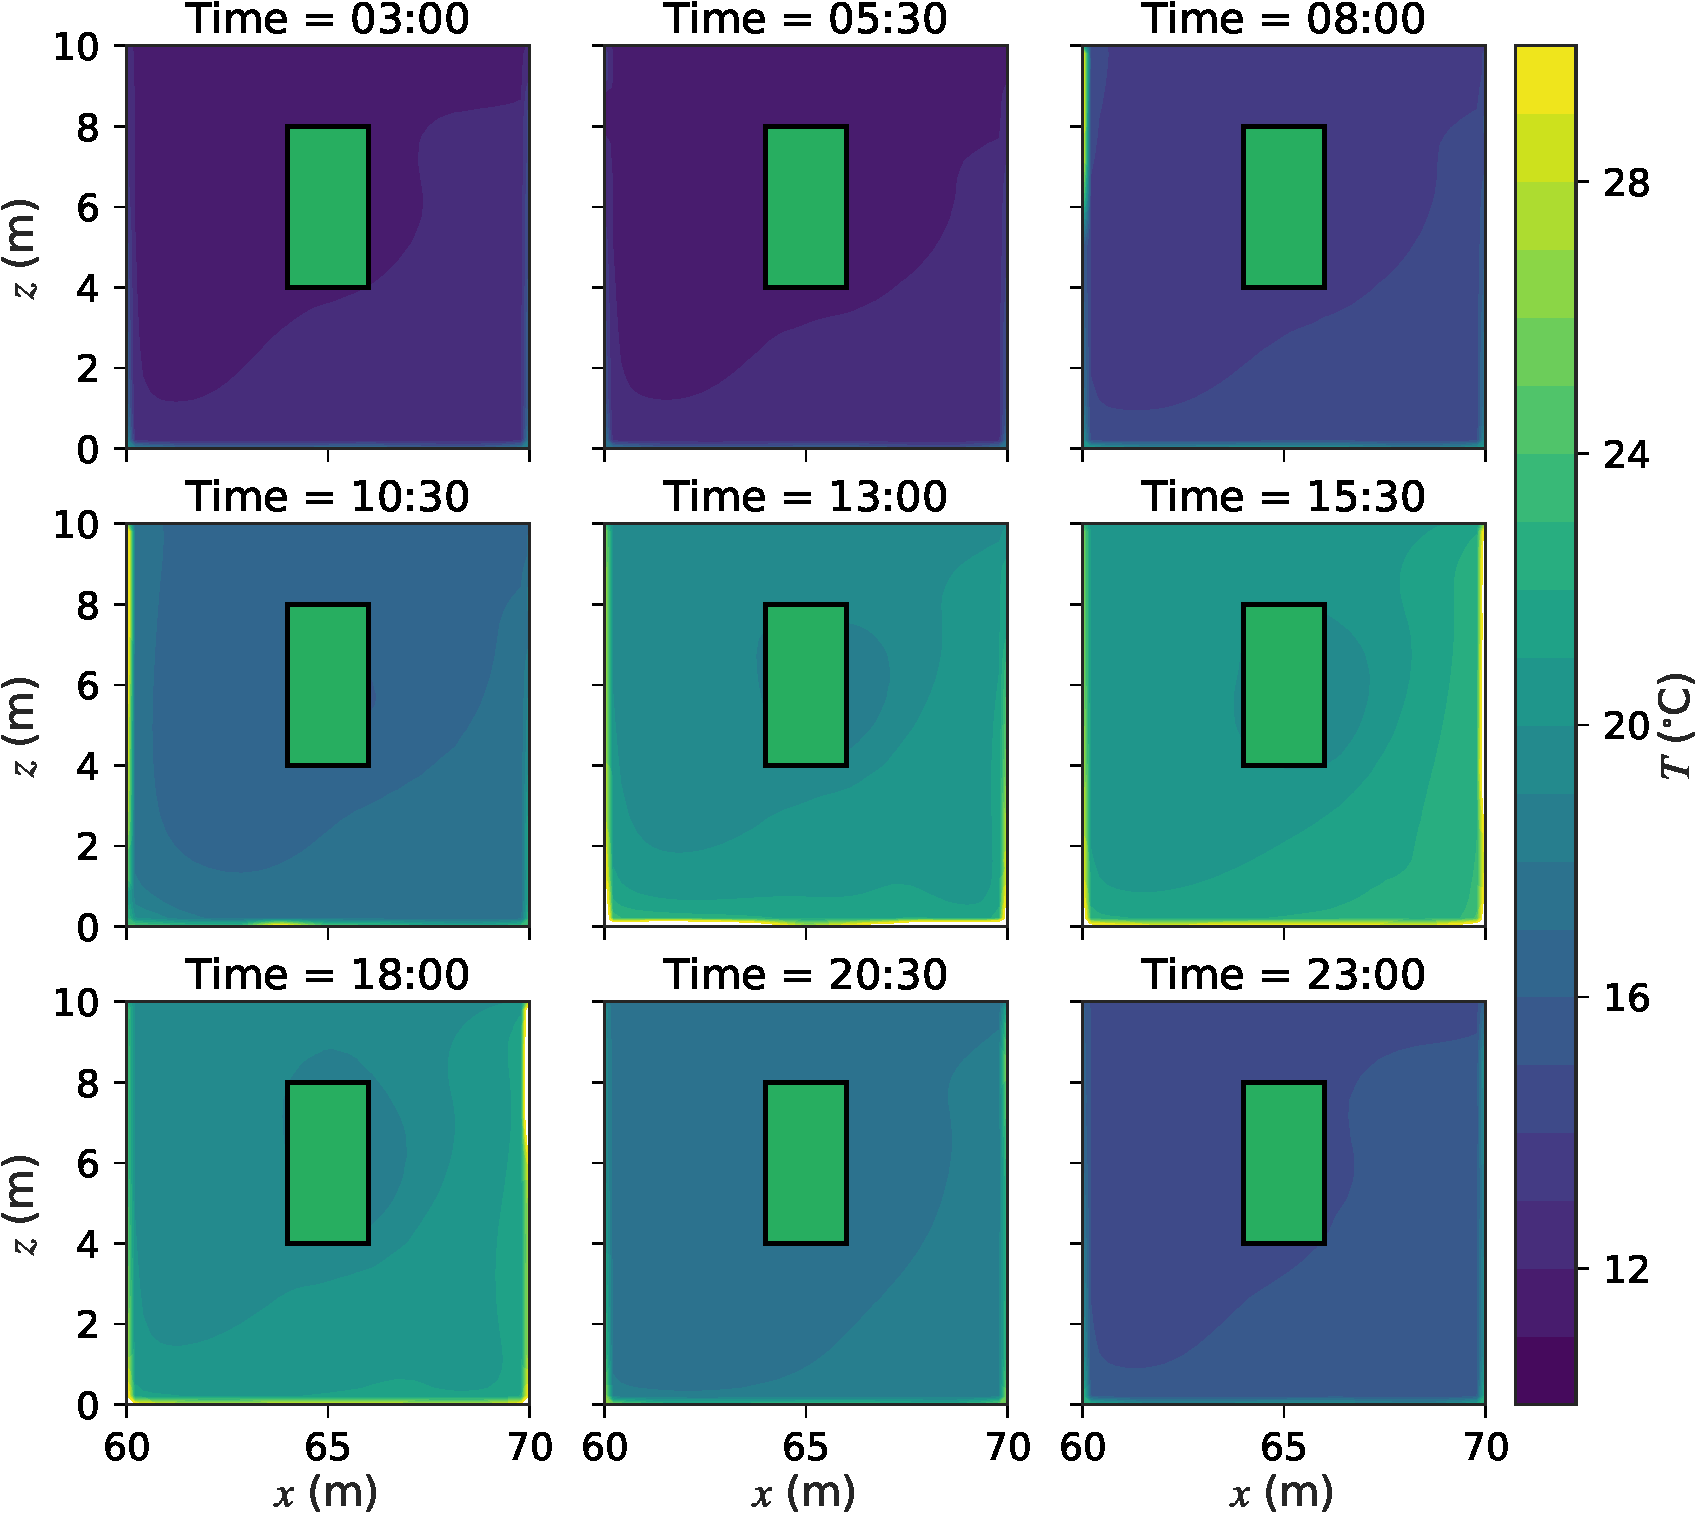
\includegraphics[width=0.8\textwidth]{\figdir/USC_T-crop.pdf}
	\caption{Air temperature $T$ ($^{\circ}$C) inside the street-canyon where the vegetation zone is indicated by a green box. The plot shows the fields with a $150$ minutes interval from $03$:$00$ (HH:MM) to $23$:$00$ (HH:MM).}
	\label{fig:USC_T}
\end{sidewaysfigure}

\cref{fig:USC_T} shows the air temperature $T$ ($^{\circ}$C) inside the street-canyon (i.e., $x-z$ plane at $y=125$ m). Therefore, is it is possible to see the influence of vegetation on the air temperature through the diurnal cycle. The air temperature $T$ depicted in the figures is resulted from the net effect of solar radiation, plant shading, thermal storage in buildings and air temperature change to plant transpiration. It is apparent that the highest air temperature is at building surfaces mainly due to the solar radiation observed in \cref{fig:USC_qrdir}. In the vicinity of the vegetation, a cooler region is prevalent and is directly due to the air temperature cooling from plant transpiration. The transpirative cooling is predominant from mid-day to afternoon (i.e., 13:00 to 18:00), when the solar radiation is present and so provides cooling when radiation intensity is highest. %However, to better assess the influence of vegetation, a single location below the tree at $(x,y,z) = (65, 125, 2)$ is cross-examined with two other cases: i) no vegetation and, ii) vegetation with only shading and no plant transpiration (\textit{Shad.}). 

%To quantify and distinguish the natural cooling associated with transpirative cooling and the natural cooling associated with tree-shade cooling, two simulation cases are compared: transpiration and shaded case (T+S) and shade only case (S). Fig. 3 compares the diurnal variation of the temperature drop, $T_v-T_nv$, for these two configurations, for a single measurement point below the row of trees at x= 65 m, y= 125 m and height of z= 2 m. The peak reduction in air temperature below the tree is seen to occur at noon, when the point is under the shadow. The configuration “S”, with only shadow, shows a peak air temperature drop of around -1.0 ℃ whereas with transpiration (T+S), an additional temperature drop of -0.2 is found. Therefore, the tree-shade cooling is dominant here. Furthermore, studying the diurnal variation, it is evident that the cooling effect of vegetation is also present during the night time, even after transpiration and tree shade are no longer present, with a temperature drop of around -0.4. This indicates that a reduction in the heat storage inside the buildings has a prolonged benefit to the urban climate.

%\subsubsection*{Influence of shading}


\subsubsection*{Impact of thermal comfort}

The influence of vegetation on pedestrian comfort is determined by evaluating the Universal Thermal Climate Index (\textit{UTCI}) ($^{\circ}$C) \citep{Fiala2001,Manickathan2018a}. We employ the formulation used in \cref{ch:parametricstudy}, however, with a more accurate estimation of the mean radiant temperature, as shown in \cref{eq:Tmrt2}, taking in account of the solar altitude change during the day, long-wave and short-wave radiation emitted and reflected from the urban surfaces. \cref{fig:USC_UTCI} shows the $\textit{UTCI}$ ($^{\circ}$C) inside the street-canyon (i.e., $x-z$ plane at $y=125$ m) at 9 periods of the days. It is apparent that the pedestrian comfort is significantly compromised due to the exposure to solar radiation at noon. However, inside the shaded zone of the trees, the thermal comfort is substantially improved, as indicated by the reduced UTCI values. In contrast, the impact of humidity generated from the trees is not discernible in the UTCI distribution. This means the transpiration of the trees does not negatively affect pedestrian comfort in the case studied, although an increase in relative humidity could reduce the thermal comfort.

% We position a pedestrian under the tree, Fig. 4 shows the diurnal variation of the UTCI for three different cases: setup without vegetation (no veg), setup with only shading vegetation (S) and setup with transpiring and shading vegetation (T+S). 

\begin{sidewaysfigure}[p]
	\centering
	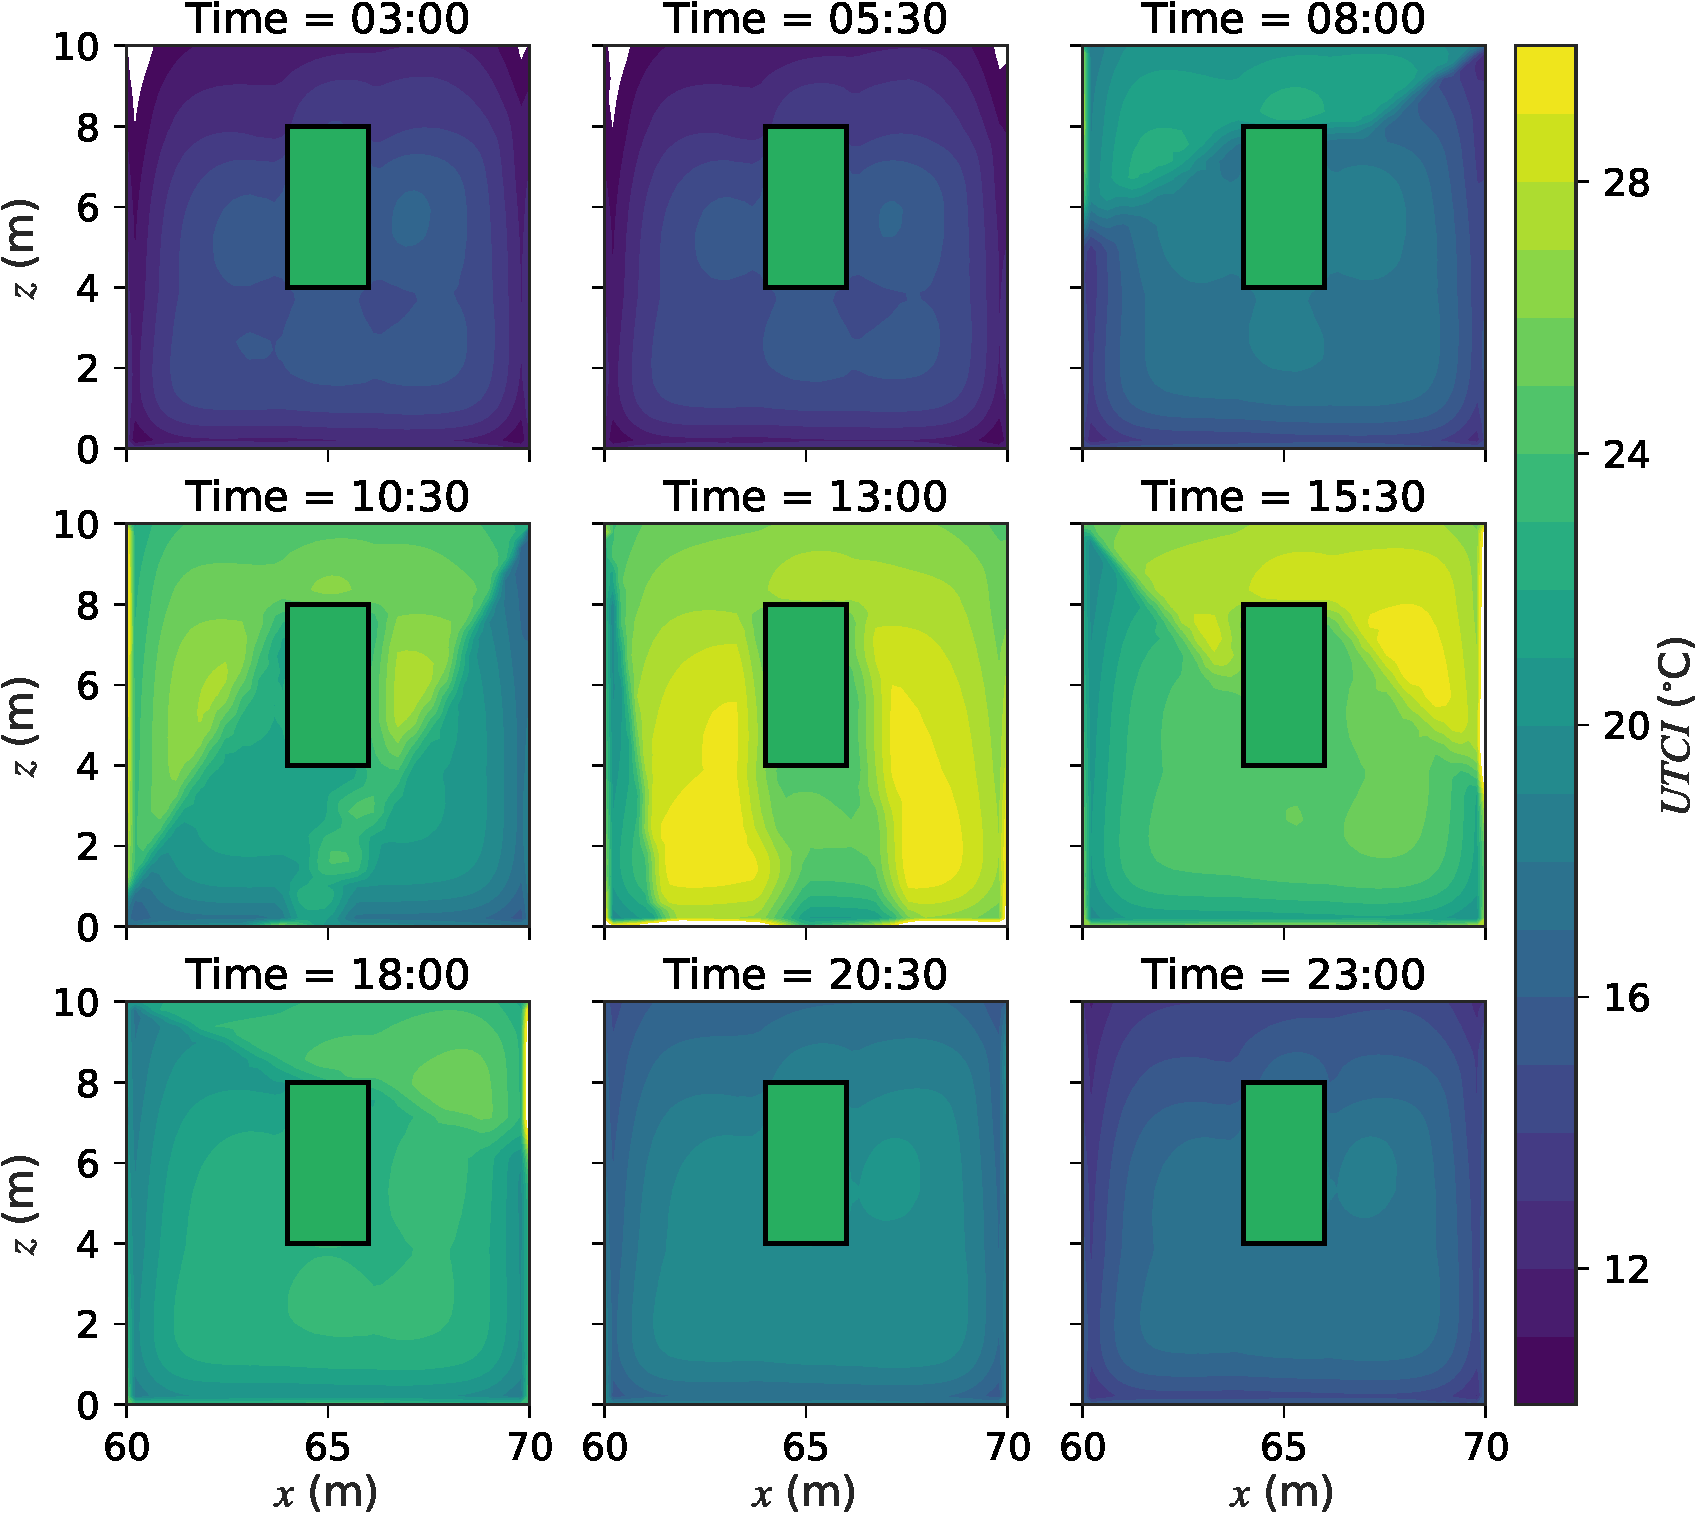
\includegraphics[width=0.8\textwidth]{\figdir/USC_UTCI-crop.pdf}
	\caption{Universal thermal climate index $\textit{UTCI}$ ($^{\circ}$C) inside the street-canyon where the vegetation zone is indicated by a green box. The plot shows the fields with a $150$ minutes interval from $03$:$00$ (HH:MM) to $23$:$00$ (HH:MM).}
	\label{fig:USC_UTCI}
\end{sidewaysfigure}

To better assess the influence of the transpiration and the influence of shading, the air temperature $T$  ($^{\circ}$C) and $UTCI$  ($^{\circ}$C) below the tree at $(x,y,z) = (65, 125, 2)$ for three different cases are studied: i) no vegetation, ii) only shading, and iii) shading and plant transpiration. \cref{fig:profile_T_UTCI} shows the diurnal variation of the air temperature and the comfort index. The calculated \textit{UTCI} shows that the comfort perceived by the pedestrian \textit{with} and \textit{without} transpiration is identical. The perceived change in comfort is simply due the change in radiative exchanges, influenced by the vegetation. So, the change in the mean radiant temperature, seen in \cref{fig:profile_qsdir_Tmrt}, plays a more important role in the thermal comfort. During night time, the UTCI with vegetation is slightly higher and is due to the higher mean radiant temperature observed in \cref{fig:profile_qsdir_Tmrt}. Due to the radiation trapping, the noctural UTCI is higher can therefore indicates a lower thermal comfort. 

\begin{figure}[t]
	\centering
	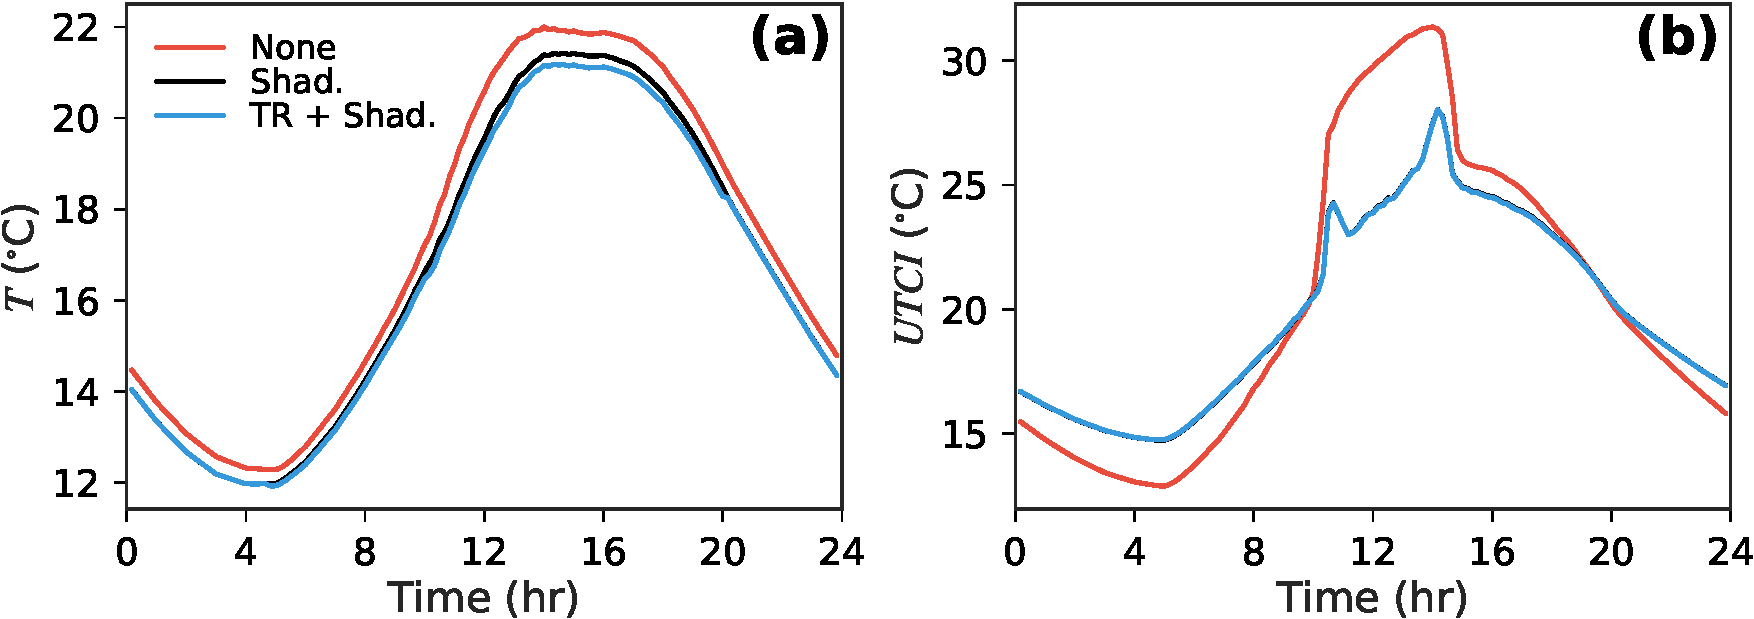
\includegraphics[width=\textwidth]{\figdir/profile_T_UTCI-crop.pdf}
	\caption{Diurnal profile below the tree at $(x,y,z) = (65, 125, 2)$ comparing three cases: no vegetation (\textit{None}), vegetation with only shading (\textit{Shad.}), and vegetation providing shading and transpirative cooling (\textit{TR + Shad.}): \subfig{a} air temperature $T$  ($^{\circ}$C) and \subfig{b} universal thermal climate index $\textit{UTCI}$ ($^{\circ}$C). }
	\label{fig:profile_T_UTCI}
\end{figure}


%The cooling potential of trees in the street canyon is quantified by studying the diurnal variations of air temperature and humidity for three distinctly different configurations: street canyon without tree, street canyon with trees but only providing shading and, finally, street canyon with trees providing both transpirative cooling and cooling due to shading. The configuration of trees that only provide shading in the street canyon is achieved by artificially closing the stomata in the model. Figure 2 shows the diurnal variation of air temperature and humidity ratio below the tree at z=2 m (point at the middle of the street canyon) for these three configurations. The figure shows that, without the trees, the air temperature is quantifiably higher throughout both day and night. However, once the trees are present, both shading and transpiration provide cooling in the street canyon, with an average decrease of 0.5°C in presence of shading and of an additional 0.2°C, when transpiration is added to shading. The cooling due to shading is seen to be higher than the cooling provided from transpiration. The study on the diurnal variation of humidity ratio inside the street canyon, Figure 2b, shows that the humidity in the street canyon is increased when the trees transpire. This could potentially negatively affect the pedestrian comfort below the tree. 


\subsubsection*{Influence of water availability}

\begin{figure}[p]
	\centering
	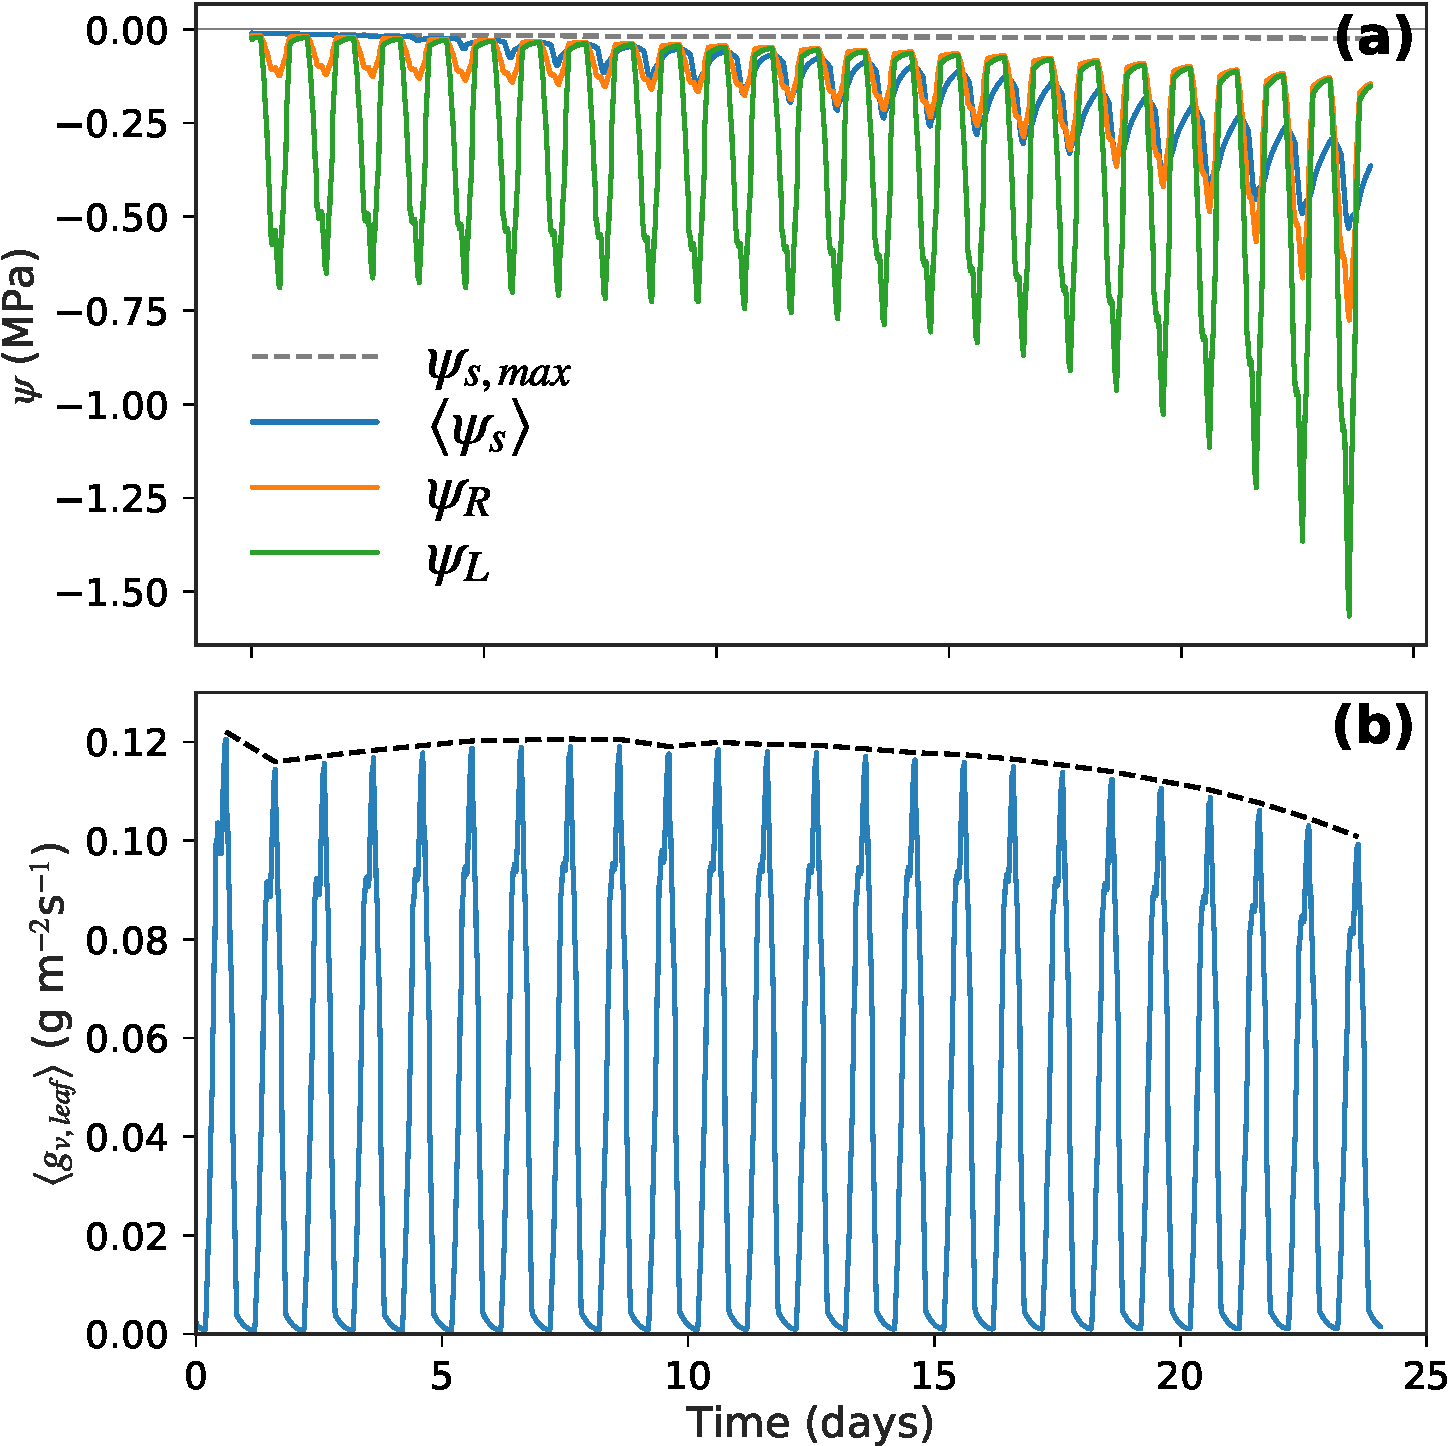
\includegraphics[width=\textwidth]{\figdir/profile_psi_gvleaf_v2-crop.pdf}
	\caption{Long-term evolution of the plant properties changing due reducing water availability simulated for $25$ days: \subfig{a} bulk leaf water potential $\psi_L$ (MPa), bulk root water potential $\psi_R$ (MPa), rhizosphere-averaged soil water potential $\langle \psi_s \rangle$ (MPa) and maximum rhizosphere soil water potential $\psi_{\textit{s,max}}$ (MPa) \subfig{b} average plant transpiration rate $\langle g_{\textit{v,leaf}} \rangle$ (g\,m$^{-2}$\,s$^{-1}$). }
	\label{fig:profile_psi_gvleaf}
\end{figure}

\begin{figure}[p]
	\centering
	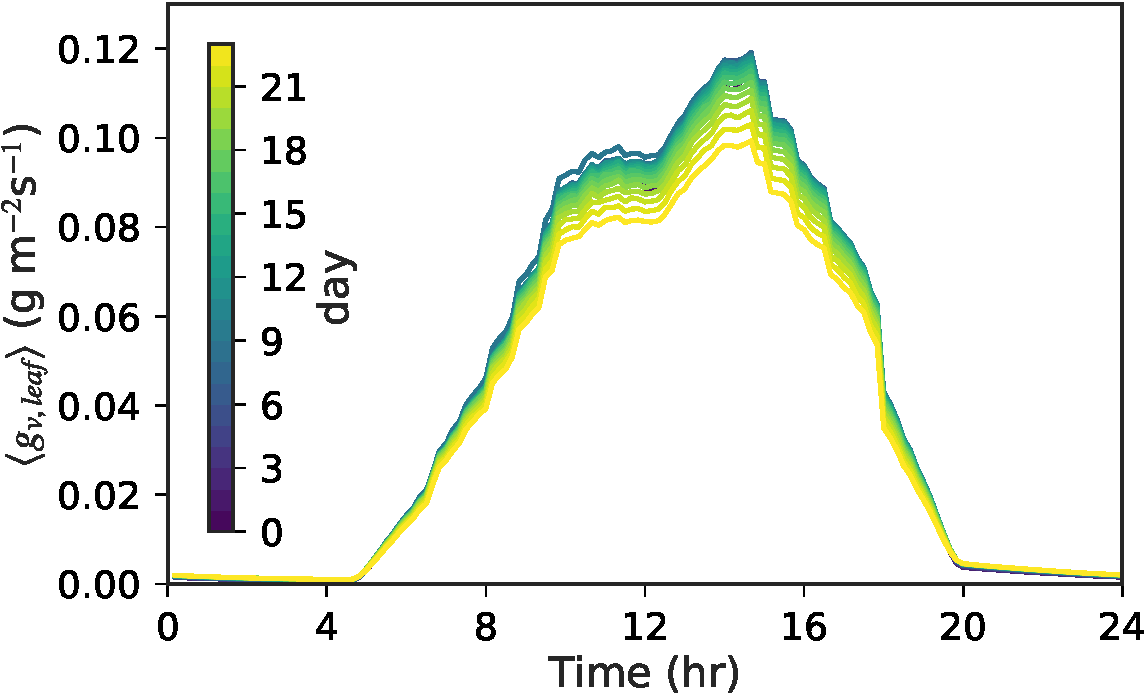
\includegraphics[width=0.8\textwidth]{\figdir/profile_gvleaf_collapsed-crop.pdf}
	\caption{Hourly variation of plant transpiration rate $\langle g_{\textit{v,leaf}} \rangle$ (g\,m$^{-2}$\,s$^{-1}$ of all 25 days.}
	\label{fig:profile_gvleaf_collapsed}
\end{figure}

\begin{figure}[p]
	\centering
	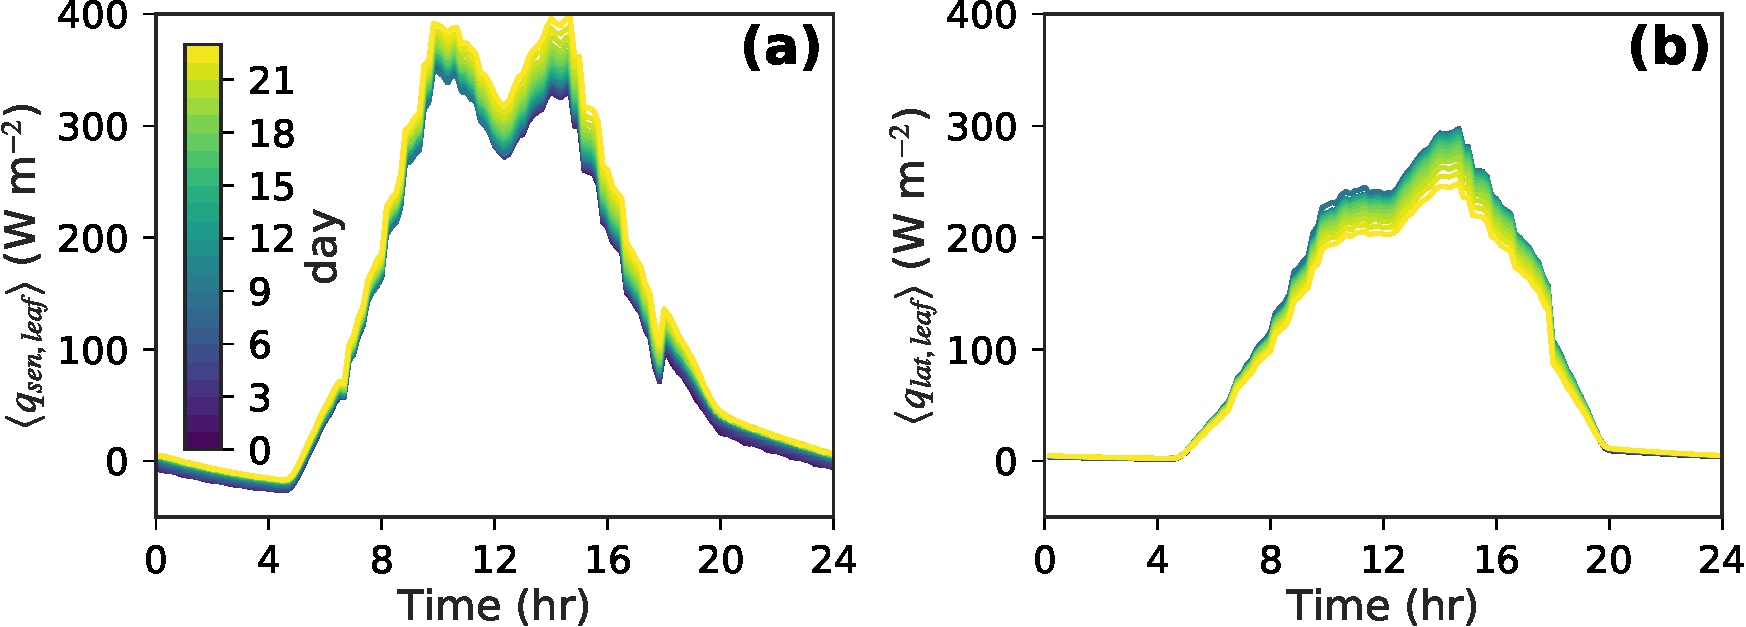
\includegraphics[width=\textwidth]{\figdir/energy_collapsed-crop.pdf}
	\caption{Hourly variation of plant energy fluxes changing due to reducing water availability: \subfig{a} average sensible heat flux $\langle q_{\textit{sen,leaf}} \rangle$ (W\,m$^{-2}$) and \subfig{b} average latent heat flux $\langle q_{\textit{lat,leaf}} \rangle$ (W\,m$^{-2}$). }
	\label{fig:energy_collapsed}
\end{figure}

A final aspect that can play a role is the water availability for the plants. As the plant transpires throughout the day, the soil moisture will reduce due to the root water uptake (in addition to soil surface evaporation). Therefore, after a longer period of time (i.e., days), the soil moisture will reduced and could have an impact on the plant transpiration rate, directly influence the leaf energy balance.  \cref{fig:profile_psi_gvleaf} shows the long-term evolution of the plant properties such as bulk leaf water potential $\psi_L$ (MPa), bulk root water potential $\psi_R$ (MPa), rhizosphere-averaged soil water potential $\langle \psi_s \rangle$ (MPa), and average plant transpiration rate $\langle g_{\textit{v,leaf}} \rangle$ (g\,m$^{-2}$\,s$^{-1}$). The rhizosphere-averaged soil water potential is defined as:
\begin{equation}
\langle \psi_s \rangle = \frac{\int_{\Omega_{\textit{soil}}} r \psi_s~\mathrm{d}V}{\int_{\Omega_{\textit{soil}}} r \mathrm{d}V }
\end{equation}
and average plant transpiration rate is defined as:
\begin{equation}
\langle g_{\textit{v,leaf}} \rangle= \frac{\int_{\Omega_{\textit{air}}} a g_{\textit{v,leaf}}~\mathrm{d}V}{\int_{\Omega_{\textit{air}}} a \mathrm{d}V }
\end{equation}

We see that leaf and root water potential varies at two timescales: i) hourly and ii) daily. The hourly cycling behavior is directly correlated with the atmospheric conditions such as the solar radiation as depicted in \cref{fig:profile_qsdir_Tmrt}. Around early afternoon (i.e., $15$:$00$), when the solar radiation is highest, the atmospheric evaporative demand (AED) is at highest, as experimently observed in \cref{ch:microclimatestudy}. A large transpiration demand is reflected by the large drop in leaf water potential (\cref{fig:profile_psi_gvleaf}a). Similarly, the root water potential becomes more negative, albeit at a lower magnitude than the leaf water potential. The soil water potential follows a similar trend with an even smaller fluctuation between day and night values. However, what is interesting is the the average noctural rhizosphere soil water potential is lower than the root water potential. As the night progresses to dawn, we see that soil water potential becomes less negative. This is the evidence of the hydraulic redistribution \citep{Volpe2013, Huang2017}. The rhizosphere region soil moisture is highest just before dawn, and is a common metric used in plant science (i.e., pre-dawn soil water potential). The night-time hydraulic redistribution occurs when the soil water potential near the surface is lower than the bulk root water potential. Therefore, the roots acts as a mechanism to redistribute the lower-ground water where the water potential is higher (i.e., more saturated), to upper layers of the rhizosphere through the roots. Therefore, the water transport is restricted to just at the rhizosphere. The advantage is the near-surface soil can be re-moisturized, improving surface evaporative cooling or alternatively, provide ecological support to ground level vegetation such as grass. The study shows the importance of deep rooted vegetation which can access the water near water table and redistribute to regions of driest soil where the soil water potential is lowest.

\cref{fig:profile_psi_gvleaf}b shows the variation in the average plant transpiration rate. The plant transpiration is correlated with the leaf water potential as they are directly dependent, with peak plant transpiration around early afternoon ($15$:$00$).  The long-term dynamics of water availability is also visible in the \cref{fig:profile_psi_gvleaf}. As the number of days passes, a larger gradient in the leaf and root water potential is required to provide the adequate transpiration needed by the atmospheric demand. Furthermore, after day 20, we observe a exponential behavior in the daily variability indicating that plants are more susceptible after an extended period of low soil moisture. Furthermore, if we quantify water stress as a difference between the leaf and soil water potential, we see that plant water stress increases exponential as the day passes. \cref{fig:profile_gvleaf_collapsed} shows the plant transpiration rate $\langle g_{\textit{v,leaf}} \rangle$ (g\,m$^{-2}$\,s$^{-1}$), where all the 25 days are collapsed to an hourly plot. We see that with increasing number of days without irrigation, the plant transpiration decays throughout the day and is proportional to the strength of the plant transpiration. So, the largest drop in plant transpiration is observed at peak solar hour.

To understand how the decaying transpiration rate affects the plant energy balance, the hourly variation of the average sensible heat flux $\langle q_{\textit{sen,leaf}} \rangle$ (W\,m$^{-2}$) and  average latent heat flux $\langle q_{\textit{lat,leaf}} \rangle$ (W\,m$^{-2}$) is investigated, \cref{fig:energy_collapsed}. The figure shows that with reducing water availability, the sensible heat flux increases throughout the day with an equal reduction in the latent heat flux. The study shows the importance of the regular irrigation of the vegetation. Without adequate irrigation, a lack of water for plant transpiration can remove the transpirative cooling effect observed in \cref{fig:profile_T_UTCI}. If the amount of water in the soil reaches the permanent wilting point $\psi = \num{-1.5e6}$ (Pa), it is known that plant can no longer transpire due to loss of cell turgidity \citep{Idso1977}. So, to ensure the health of the plant, it is crucial plants are irrigated. The study showed that, with increasing number of days (for the previous irrigation), the need for irrigation grows exponentially as reflected by the water stress.

Finally, the influence of water availability on the thermal comfort is not observable. This is because, the $UTCI$  ($^{\circ}$C) is identical as shown in \cref{fig:profile_T_UTCI}b. This is because, the shading provided by vegetation plays a more important role on the thermal comfort. However, an interesting aspect that could be investigated is the influence of water availability on the leaf area density $a$. A wilting of the plant could potential reduce the shadowing provided by vegetation, which can influence the thermal comfort. However, in the present study this aspect is not investigated.

\subsection{Conclusion}

The present study investigates the influence of transpirative and tree shading on the microclimate of a street canyon. The study shows that transpiration has a direct influence in the plant vicinity air temperature and negligible effects the thermal comfort measured through Universal Thermal Climate Index (UTCI). In contrast, the shading provided by vegetation has a large influence on the street-canyon mean radiant temperature with a drop of around $18$ ($^{\circ}$C) in the shadow. A large drop in the mean radiant temperature substantially improves the measured thermal comfort. An important aspect of vegetation that should be taken int account is the noctural radiation trapping due to presence of vegetation. At night, due to obstruction of long-wave radiation emission from urban surfaces to the sky, the mean radiant temperature and equally UTCI, is higher during night time. This indicates that vegetation counter-intuitively stagnates the cooling of cities during night. So cities to not ignore this contribution of vegetation when employing UHI mitigation measures using vegetation.

Another aspect that also plays an important role is the water availability. With increasing number of days without irrigation, the soil loses the available water for the plant transpiration. We observed that due to this, the transpiration rate decays, resulting in an increase in the sensible heat flux from vegetation. Furthermore, a prolonged period without irrigation is shown to increase the water stress of the plant (i.e., difference between leaf and soil water potential), which increases at an exponential rate. Therefore, the demand for irrigation also grows exponential with time. Urban vegetation irrigation measure should therefore take in account of the growth in water stress when exposed prolonged period of drought that could arise in today's changing climate. Finally, the complex modeling approach implemented in this study is able to capture import plant dynamics such as hydraulic redistribution. This can have important contribution to the water availability of the shallow-rooted plant species such as grass or small shrubs.

\section{Case study: Muensterhof}

\subsection{Simulation setup}


\begin{sidewaysfigure}[p]
	\centering
	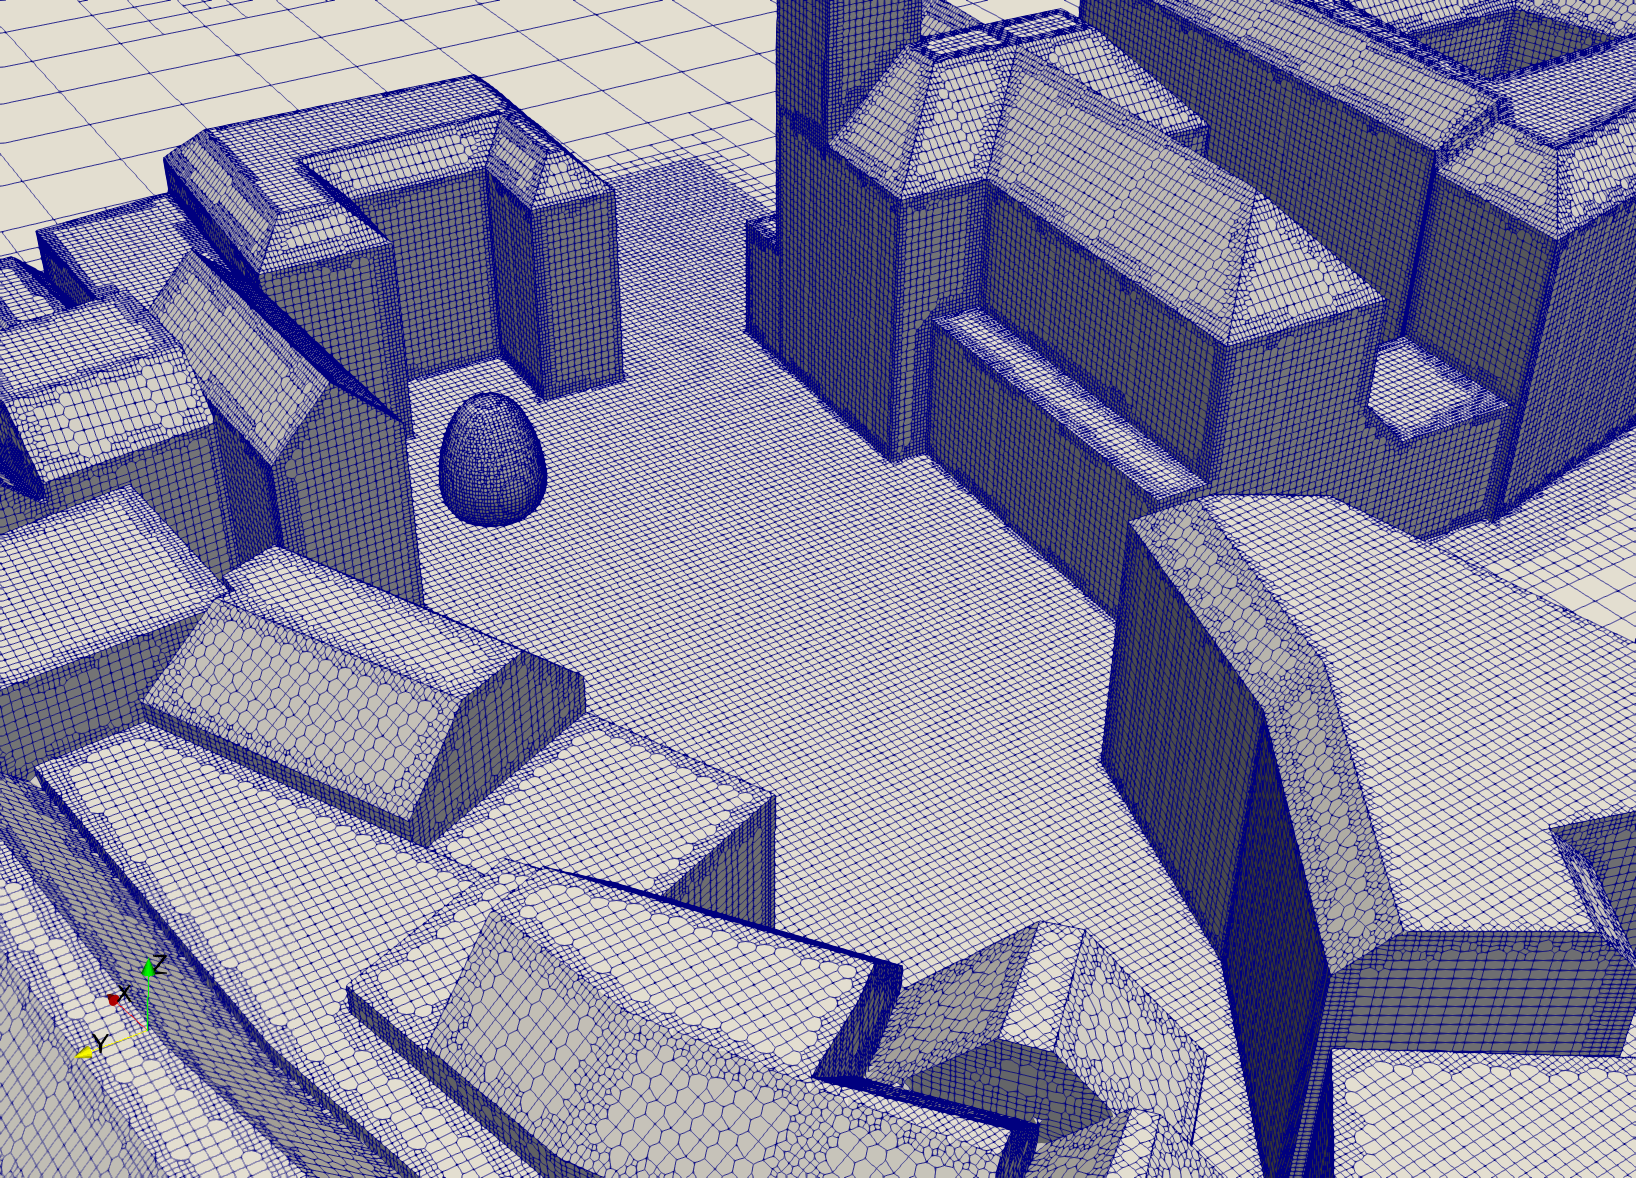
\includegraphics[width=0.8\textwidth]{\figdir/mesh_resolution_muensterhof_tree_V2.png}
	\caption{Simulation sub-domain showing the surface layer mesh refined closed to the building walls in Muensterhof along with a single isolated tree. The numerical domain is discretized into $\num{4432297}$ cells with minimum cell size of $\num{2.38e-3}$ m$^{3}$ near the building.}
	\label{fig:mesh_resolution_muensterhof_tree}
\end{sidewaysfigure}


\subsection{Results and Discussion}

\subsection{Conclusion}
